%% LyX 2.3.1 created this file.  For more info, see http://www.lyx.org/.
%% Do not edit unless you really know what you are doing.
\documentclass[english]{article}
\usepackage[T1]{fontenc}
\usepackage[utf8]{inputenc}
\usepackage{geometry}
\geometry{verbose,tmargin=2cm,bmargin=2cm,lmargin=1cm,rmargin=1cm,footskip=1cm}
\pagestyle{empty}
\setlength{\parskip}{0mm}
\setlength{\parindent}{0pt}
\usepackage{babel}
\usepackage{mathrsfs}
\usepackage{amsmath}
\usepackage{amssymb}
\usepackage{graphicx}
\usepackage{wasysym}
\usepackage{esint}
\PassOptionsToPackage{normalem}{ulem}
\usepackage{ulem}
\usepackage[unicode=true,
 bookmarks=false,
 breaklinks=false,pdfborder={0 0 1},backref=section,colorlinks=false]
 {hyperref}

\makeatletter

%%%%%%%%%%%%%%%%%%%%%%%%%%%%%% LyX specific LaTeX commands.
%% Because html converters don't know tabularnewline
\providecommand{\tabularnewline}{\\}

%%%%%%%%%%%%%%%%%%%%%%%%%%%%%% User specified LaTeX commands.
\usepackage{babel}

\makeatother

\begin{document}
\title{Fisica Generale T-2}
\author{Urbinati Cristian}
\date{21/09/2018}

\maketitle
 
\begin{center}
\href{mailto:cristian.urbinati@studio.unibo.it}{e-mail: cristian.urbinati@studio.unibo.it}
\par\end{center}

\begin{center}
\href{https://github.com/urbinaticri/Unibo_computerEngineeringNotes}{Altro : https://github.com/urbinaticri/Unibo\_computerEngineeringNotes}
\par\end{center}

\begin{center}
Materiale distribuito con licenza \href{https://creativecommons.org/licenses/by-nc-sa/2.0/it/}{Creative Commons}
\par\end{center}

\begin{center}
Attribuzione - Non commerciale - Condividi allo stesso modo 2.0 Italia
(CC BY-NC-SA 2.0 IT) 
\par\end{center}

\begin{center}
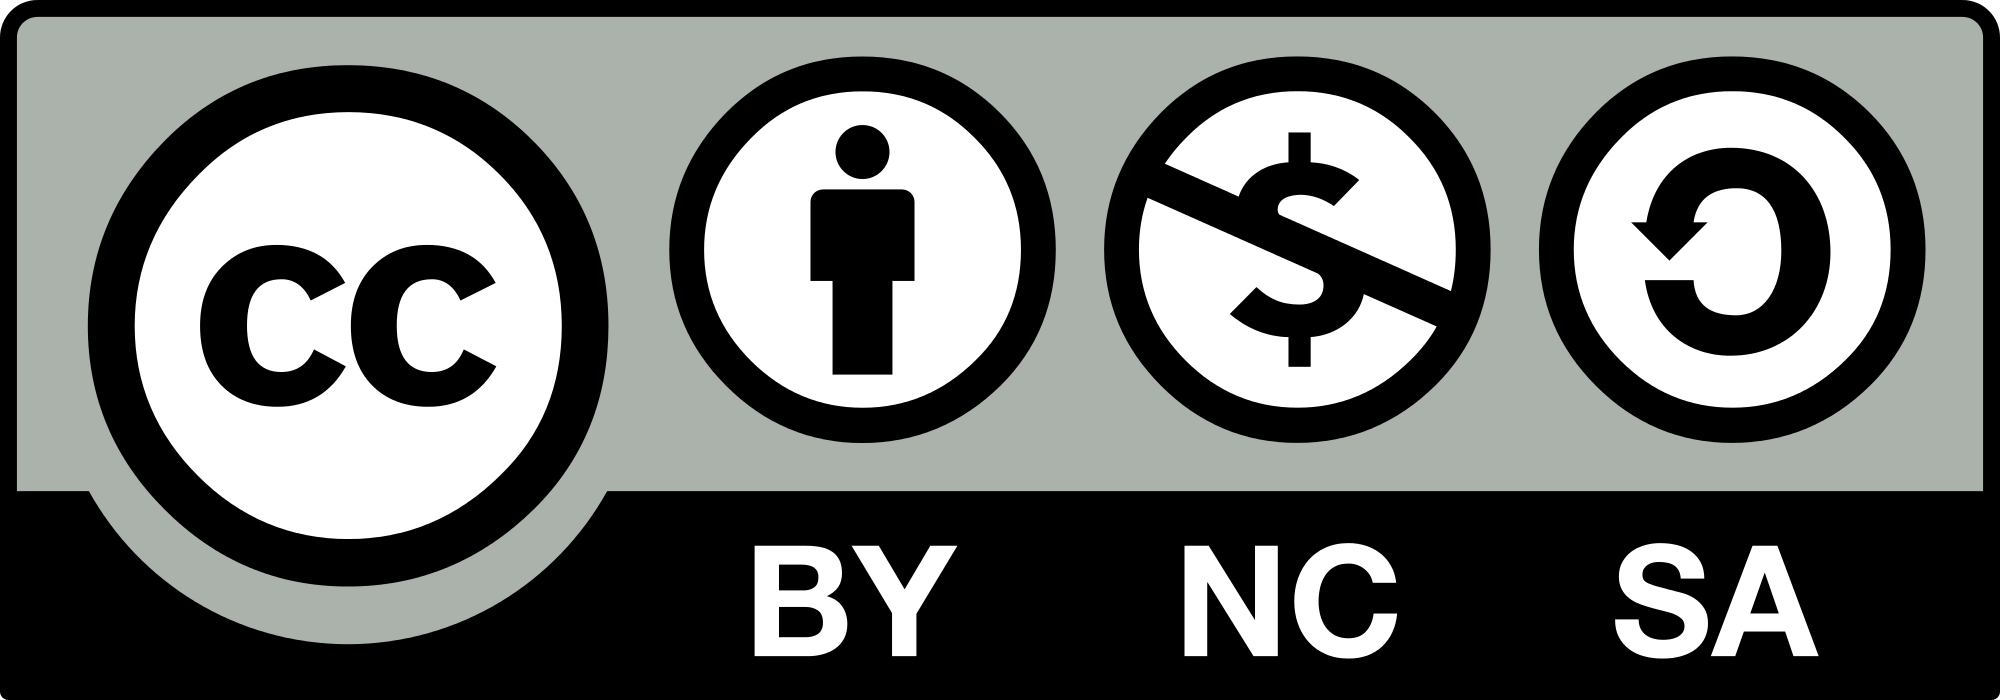
\includegraphics[scale=0.05]{img/CreativeCommonsLicense} 
\par\end{center}

\pagebreak{}

\section{Elettrostatica}

\subsection*{Introduzione}

L'elettrostatica è una branca dell'elettromagnetismo che studia le
cariche elettriche in condizioni di equilibrio.

L'unità di misura della carica nel S.I. è il Coulomb (C) dove $\text{C}=\text{A}\cdot\text{s}\quad\text{(Ampere}\cdot\text{secondi)}$. 

Si parla di \textbf{elettrizazione vetrosa }se la carica elettrica
è positiva.

Si parla di \textbf{elettrizzazione resinosa} se la carica elettrica
è negativa.

Carica elettrica elementare: $\left|q_{e}\right|=1.6\times10^{-19}C$

In un sistema isolato, la carica elettrica si conserva.

\subsection*{Legge di Coulomb}

La forza elettrostatica esercitata dalla carica $q_{1}$ sulla carica
$q_{2}$ è 
\[
\vec{F}_{12}=\frac{1}{4\pi\varepsilon_{0}}\frac{q_{1}q_{2}}{r^{2}}\hat{r}
\]

dove $\varepsilon_{0}=8.85\times10^{-12}\frac{\text{C}^{2}}{\text{N}\text{m}^{2}}\,\left(\frac{\text{F}}{\text{m}}\right)$

\subsection*{Principio di sovrapposizione}

In un sistema di $N$ cariche puntiformi la forza totale sulla carica
$q$ è la somma vettoriale delle forze che le cariche $q_{i}$ eserciterebbero
singolarmente su $q$ se $q_{j\neq i}$ fossero assenti:

\[
\vec{F}=\sum_{i=1}^{N}\vec{F}_{i}=\sum_{i=1}^{N}\frac{1}{4\pi\varepsilon_{0}}\frac{qq_{i}}{r_{i}^{2}}\hat{r}
\]

dove $\vec{r}_{i}$ è il vettore posizionale da $q_{i}$ a $q$.

\subsection*{Campo elettrico di una carica puntiforme}

Il campo elettrico è un campo vettoriale $P\left(\in\mathbb{R}^{3}\right)\longrightarrow\vec{E}\left(P\right)$
con $\vec{E}\left(\vec{r}\right)=\frac{1}{4\pi\varepsilon_{0}}\frac{Q}{r^{2}}\hat{r}$.
\begin{center}
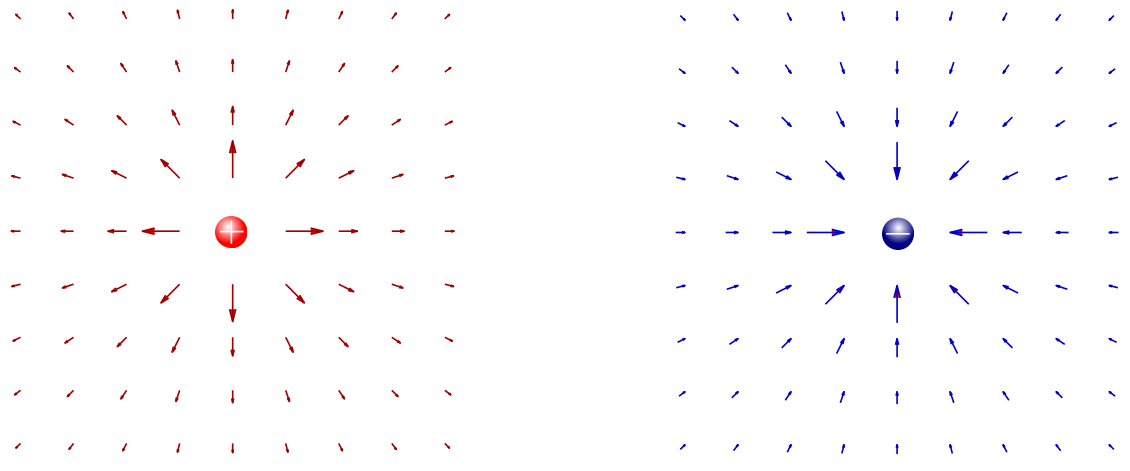
\includegraphics[scale=0.25]{img/Campo_elettrostatico_di_una_carica_elementare}
\par\end{center}

\subsubsection*{Riformulazione della forza di Coulomb}

\[
\vec{F}=\sum_{i=1}^{N}\vec{F}_{i}=q\sum_{i=1}^{N}\frac{1}{4\pi\varepsilon_{0}}\frac{q_{i}}{r_{i}^{2}}\hat{r}=q\vec{E}
\]

dove $\vec{E}$ è il campo elettrico generato da una carica $Q={\displaystyle \sum_{i=0}^{N}q_{i}}$.
\begin{center}
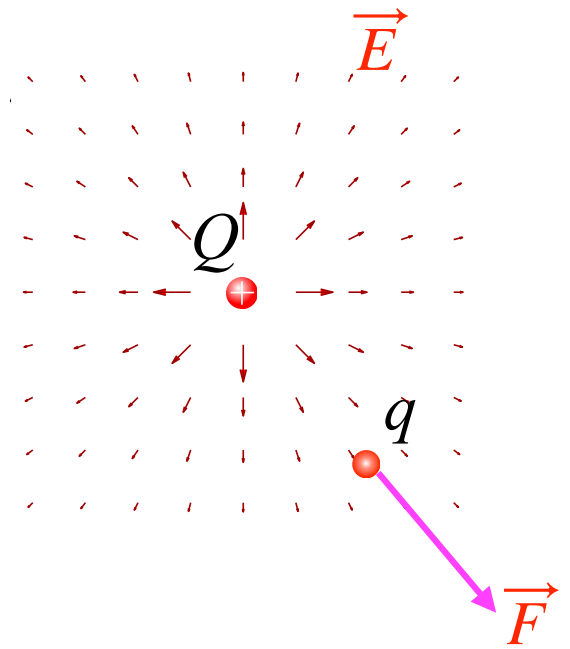
\includegraphics[scale=0.2]{img/Riformulazione_legge_di_Coulomb_con_campo_elettrostatico}
\par\end{center}

\subsection*{Distribuzione continua di carica}
\begin{center}
\begin{tabular}{|c|c|c|}
\hline 
\textbf{Densità di carica volumetrica} & \textbf{Carica volume elementare} & \textbf{Carica volume}\tabularnewline
\hline 
\multicolumn{1}{c}{$\rho={\displaystyle \lim_{\Delta\tau\rightarrow0}}\frac{\Delta q}{\Delta\tau}=\frac{\text{d}q}{\text{d}\tau}$} & \multicolumn{1}{c}{$dq=\rho\text{d}\tau$} & \multicolumn{1}{c}{$q_{\tau}=\iiint_{\tau}\rho\text{d}\tau$}\tabularnewline
\end{tabular}
\par\end{center}

\begin{center}
\begin{tabular}{|c|c|c|}
\hline 
\textbf{Densità di carica superficiale} & \textbf{Carica superficie elementare} & \textbf{Carica superficie}\tabularnewline
\hline 
\multicolumn{1}{c}{$\sigma={\displaystyle \lim_{\Delta S\rightarrow0}}\frac{\Delta q}{\Delta S}=\frac{\text{d}q}{\text{d}S}$} & \multicolumn{1}{c}{$dq=\sigma\text{d}S$} & \multicolumn{1}{c}{$q_{S}=\iint_{S}\sigma\text{d}S$}\tabularnewline
\end{tabular}
\par\end{center}

\begin{center}
\begin{tabular}{|c|c|c|}
\hline 
\textbf{Densità di carica lineare} & \textbf{Carica linea elementare} & \textbf{Carica linea}\tabularnewline
\hline 
\multicolumn{1}{c}{$\lambda={\displaystyle \lim_{\Delta l\rightarrow0}}\frac{\Delta q}{\Delta l}=\frac{\text{d}q}{\text{d}l}$} & \multicolumn{1}{c}{$dq=\lambda\text{d}l$} & \multicolumn{1}{c}{$q_{l}=\int_{l}\lambda\text{d}l$}\tabularnewline
\end{tabular}
\par\end{center}

\begin{center}
\begin{tabular}{ccc}
\hline 
\multicolumn{1}{|c|}{\textbf{Carica distribuita su volume}} & \multicolumn{1}{c|}{\textbf{Carica distribuita su superficie}} & \multicolumn{1}{c|}{\textbf{Carica distribuita su linea}}\tabularnewline
\hline 
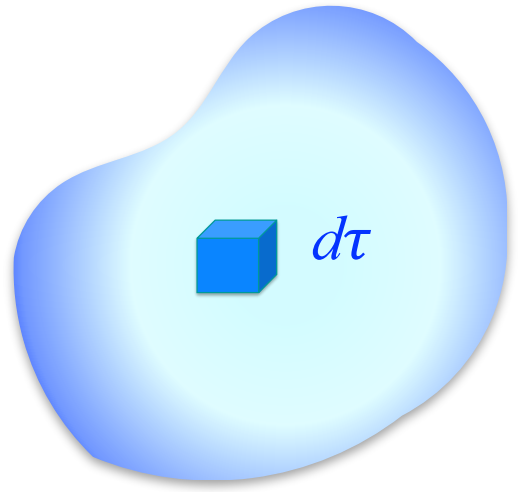
\includegraphics[scale=0.15]{img/Densita_carica_volumetrica} & 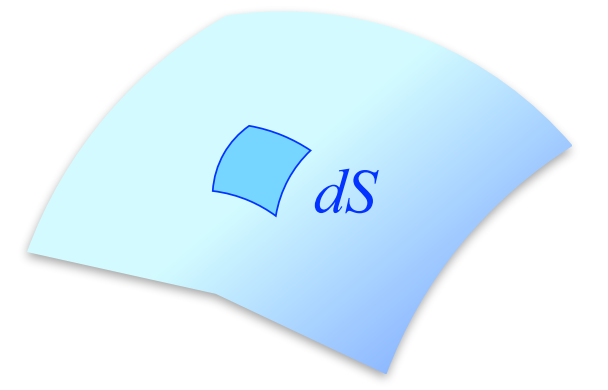
\includegraphics[scale=0.2]{img/Densita_carica_superficiale} & 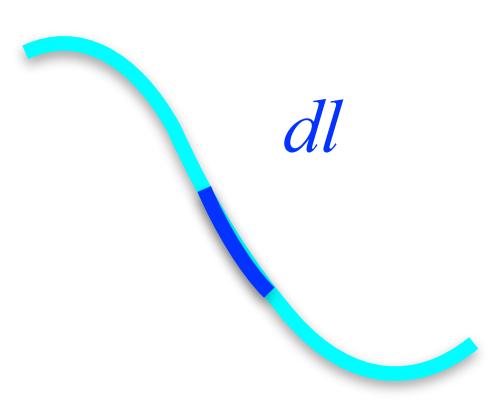
\includegraphics[scale=0.2]{img/Densita_carica_lineare}\tabularnewline
$\vec{E}\left(\vec{r}\right)=\frac{1}{4\pi\varepsilon_{0}}{\displaystyle \iiint_{\tau}\frac{\rho\left(\vec{r'}\right)\left(\vec{r}-\vec{r'}\right)}{\left|\vec{r}-\vec{r'}\right|^{3}}\text{d}\tau}$ & $\vec{E}\left(\vec{r}\right)=\frac{1}{4\pi\varepsilon_{0}}{\displaystyle \iint_{S}\frac{\sigma\left(\vec{r'}\right)\left(\vec{r}-\vec{r'}\right)}{\left|\vec{r}-\vec{r'}\right|^{3}}\text{d}S}$ & $\vec{E}\left(\vec{r}\right)=\frac{1}{4\pi\varepsilon_{0}}{\displaystyle \int_{l}\frac{\lambda\left(\vec{r'}\right)\left(\vec{r}-\vec{r'}\right)}{\left|\vec{r}-\vec{r'}\right|^{3}}\text{d}l}$\tabularnewline
\end{tabular}
\par\end{center}

\pagebreak{}

\subsection*{Integrale di superficie di una funzione vettoriale}

Siano date in $\mathbb{R}^{3}$ una funzione vettoriale $\vec{F}\left(x,y,z\right)$.
L'integrale di superficie di $\vec{F}$ è definito come:

\[
\iint_{S}\vec{F}\cdot\hat{n}\text{d}S
\]

dove $\text{d}S$ è una sezione infinitesimamente piccola della superficie
$S$.
\begin{center}
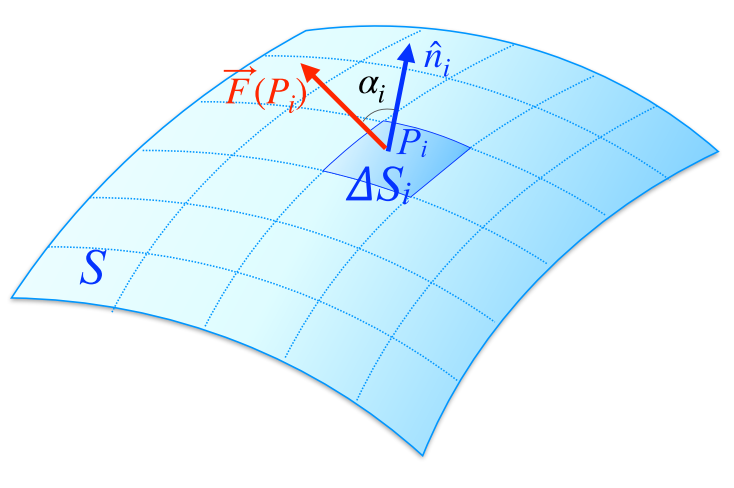
\includegraphics[scale=0.2]{img/Definizione_integrale_di_superficie}
\par\end{center}

\subsection*{Il flusso del campo elettrico}

Il campo elettrico può essere rappresentato graficamente mediante
le \textbf{linee di campo}:
\begin{center}
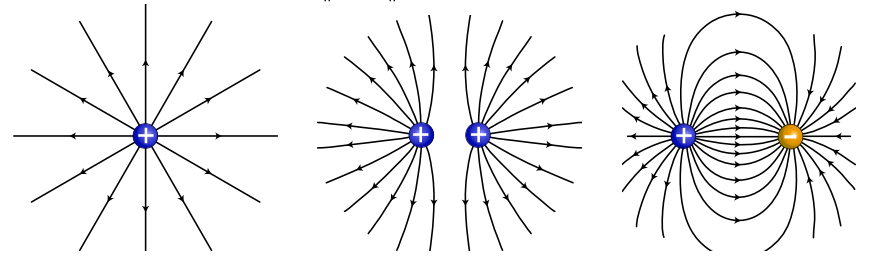
\includegraphics[scale=0.3]{img/Linee_di_flusso}
\par\end{center}

Per flusso si intende il numero di linee di campo che attraversano
una certa superficie orientata $S$. Esso è proporzionale alla grandezza
della superficie e al modulo del campo elettrico.

Osservazione: Se la superficie è parallela al campo elettrico il numero
di linee di campo che attraverserà la superficie sarà $0$ e dunque
il flusso sarà nullo. 

Il flusso infinitesimo del campo elettrico attraverso una superficie
infinitesimale $\text{d}S$ è:

\[
\text{d}\Phi_{S}\left(\vec{E}\right)=\vec{E}\cdot\hat{n}\text{d}S=E\text{d}S\cos\alpha=E\text{d}\Sigma
\]

Se consideriamo una superficie estesa $S$:

\[
\Phi_{S}\left(\vec{E}\right)=\iint_{S}\vec{E}\cdot\hat{n}\text{d}S=\iint_{S}E\text{d}S\cos\alpha=\iint_{S}E\text{d}\Sigma
\]

Se consideriamo una superficie chiusa $S$ contenente al suo interno
una carica elettrica puntiforme $q$, sapendo che l'angolo solido
è dato dalla formula $\Omega=\frac{\Sigma}{r^{2}}\in\left[0,4\pi\right]$
dove $\Sigma$ è la superficie sferica:

\[
\Phi_{S}\left(\vec{E}\right)=\oiint_{S}\vec{E}\cdot\hat{n}\text{d}S=\oiint_{S}E\underset{r^{2}\text{d}\Omega}{\underbrace{\text{d}\Sigma}}=\frac{q}{4\pi\varepsilon_{0}}\oiint_{S}\text{d}\Omega=\frac{q}{\varepsilon_{0}}
\]


\subsubsection*{Legge di Gauss del campo elettrico}

Se all'interno della superficie \uline{chiusa} $S$ ci sono $N$
cariche $q_{i}$ puntiformi, per il principio di sovrapposizione del
campo elettrico, il flusso vale:

\[
\Phi_{S}\left(\vec{E}\right)=\oiint_{S}\vec{E}\cdot\hat{n}\text{d}S=\frac{Q}{\varepsilon_{0}}\qquad Q=\sum q_{\text{int}}\equiv\iiint_{\tau(S)}\rho\text{d}\tau
\]

Oss: Il campo elettrico dipende unicamente dalla carica interna poichè
nel caso delle cariche esterne alla supericie chiusa, il numero di
linee di campo che entrano nella superficie è uguale al numero di
linee di campo che escono e quindi vi è un apporto al flusso nullo:

\[
\text{d}\Phi_{S_{1}}\left(\vec{E}_{2}\right)+\text{d}\Phi_{S_{2}}\left(\vec{E}_{2}\right)=\vec{E}_{1}\cdot\hat{n}_{1}\text{d}S_{1}+\vec{E}_{2}\cdot\hat{n}_{1}\text{d}S_{1}=E_{1}\text{d}S_{1}\cos\alpha_{1}+E_{2}\text{d}S_{2}\cos\alpha_{2}=E_{1}\left(-\text{d}\Sigma_{1}\right)+E_{2}\left(\text{d}\Sigma_{2}\right)=0
\]

\pagebreak{}

\subsection*{Divergenza di un campo vettoriale}

Consideriamo il flusso di un campo vettoriale $\vec{E}$ attraverso
una superficie chiusa $S$ che delimita un volume $\tau$:

\[
\Phi_{S}\left(\vec{E}\right)=\oiint_{S}\vec{E}\cdot\hat{n}\text{d}S
\]

Siano $S_{1}$ e $S_{2}$ le superfici chiuse che delimitano $\tau_{1}$
e $\tau_{2}$. Possiamo riscrivere il flusso come:

\[
\Phi_{S}\left(\vec{E}\right)=\oiint_{S_{1}}\vec{E}\cdot\hat{n}\text{d}S_{1}+\oiint_{S_{2}}\vec{E}\cdot\hat{n}\text{d}S_{2}
\]

Se ora invece supponiamo di dividere il volume $\tau$ in $N$ volumi
$\tau_{i}$ limitati dalle superfici chiuse $S_{i}$ avremo che: 
\[
\Phi_{S}\left(\vec{E}\right)=\sum_{i=1}^{N}\Phi_{S_{i}}\left(\vec{E}\right)\qquad\text{dove}\quad\Phi_{S_{i}}\left(\vec{E}\right)=\oiint_{S_{i}}\vec{E}\cdot\hat{n}_{i}\text{d}S_{i}
\]

Chiamiamo divergenza di un campo vettoriale il flusso uscente per
unità di volume, espresso come:

\[
\text{div}\vec{E}=\lim_{\tau_{i}\rightarrow0}\frac{\Phi_{S_{i}}\left(\vec{E}\right)}{\tau_{i}}
\]


\subsubsection*{Teorema della divergenza}

Il flusso di un campo vettoriale attraverso una superficie $S$ chiusa
è pari all'integrale sul volume $\tau$ delimitato da $S$ della divergenza
di tale campo vettoriale:

\[
\Phi_{S}\left(\vec{E}\right)=\oiint_{S}\vec{E}\cdot\hat{n}\text{d}S=\iiint_{\tau}\text{div}\vec{E}\text{d}\tau
\]


\subsubsection*{Legge di Gauss in forma locale}

Combinando il teorema della divergenza e la legge di Gauss, \uline{se
la carica è distribuita uniformemente} si ha:

\[
\text{div}\vec{E}=\frac{\rho}{\varepsilon_{0}}
\]


\subsubsection*{Significato fisico della divergenza}

La divergenza ci da un'informazione sul comportamento locale delle
linee di campo, esse:
\begin{itemize}
\item \textbf{convergono} nel punto se $\text{div}\vec{E}<0$
\item \textbf{divergono} nel punto se $\text{div}\vec{E}>0$
\end{itemize}

\subsubsection*{Divergenza in coordinate cartesiane}

\[
\text{div}\vec{F}=\vec{\nabla}\cdot\vec{F}
\]


\subsection*{Rotore}

\subsubsection*{Teorema di Stokes}

Il flusso del rotore di un campo vettoriale attraverso una superficie
$S$ aperta e orientata è uguale alla circuitazione del campo vettoriale
lungo il bordo $\Gamma$ di tale superficie:

\[
\iint_{S\left(\Gamma\right)}\left(\vec{\nabla}\wedge\vec{F}\right)\cdot\hat{n}\text{d}S=\oint\vec{F}\cdot\text{d}\vec{l}
\]

\pagebreak{}

\subsection*{Campi conservativi}

Un campo vettoriale $\vec{F}$ è conservativo se:
\begin{enumerate}
\item detto $\varphi=\underset{\Gamma}{\int}\vec{F}\cdot\text{d}\vec{l}$
allora $\underset{\Gamma\;}{\int_{A}^{B}}\vec{F}\cdot\text{d}\vec{l}=\varphi\left(B\right)-\varphi\left(A\right)$
\item $\underset{\Gamma}{\oint}\vec{F}\cdot\text{d}\vec{l}=0\quad\forall\Gamma$
\item $\vec{\nabla}\wedge\vec{F}=\vec{0}$
\item $\exists\varphi:\vec{F}=-\vec{\nabla}\varphi$
\end{enumerate}

\subsubsection*{Circuitazione del campo elettrostatico}

La circuitazione del campo lungo la linea chiusa $\Gamma$data dalla
circonferenza di raggio $r$ e centrata in $Q$ è nulla:

\[
\underset{\Gamma}{\oint}\vec{E}\cdot\text{d}\vec{l}=\underset{\Gamma}{\oint}\frac{Q}{4\pi\varepsilon_{0}r^{2}}\underset{0}{\underbrace{\hat{r}\cdot\hat{t}}}\text{d}\vec{l}=0
\]

\begin{center}
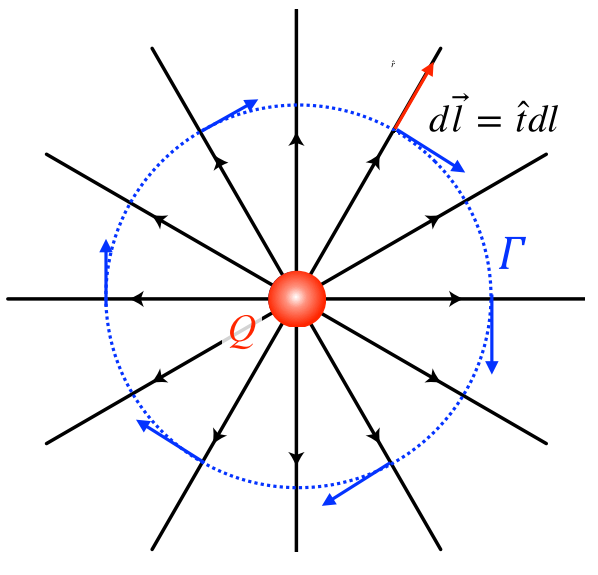
\includegraphics[scale=0.3]{img/Circuitazione_del_campo_elettrico}
\par\end{center}

Per cui il campo elettrico generato da una carica puntiforme ferma
è conservativo e dunque eredita le proprietà dei campi conservativi:
\begin{enumerate}
\item $\underset{\Gamma\;}{\int_{A}^{B}}\vec{E}\cdot\text{d}\vec{l}=V\left(B\right)-V\left(A\right)$
dove $V$ è il \textbf{potenziale elettrostatico}
\item $\underset{\Gamma}{\oint}\vec{E}\cdot\text{d}\vec{l}=0\quad\forall\Gamma$
\item $\vec{\nabla}\wedge\vec{E}=\vec{0}$ è irrotazionale (non esistono
linee di campo chiuse su loro stesse)
\item $\vec{E}=-\vec{\nabla}V$
\end{enumerate}
\pagebreak{}

\subsection*{Il potenziale elettrostatico}

Il potenziale elettrostatico $V$ è una funzione scalare in $\mathbb{R}^{3}$.
Dato un campo elettrostatico, operativemente il potenziale si calcola
integrando il differenziale esatto $\text{d}V=-\vec{E}\cdot\text{d}\vec{l}$.
L'unità di misura del potenziale nel S.I. è il Volt (V) dove

$\text{V}=\text{J}/\text{C}\quad\text{(Joule}/\text{Coloumb)}$.

L'integrale indefinito lungo una generica curva $\Gamma$ del differenziale
esatto del potenziale vale:

\[
V\left(\vec{r}\right)=-\underset{\Gamma}{\int}\vec{E}\cdot\text{d}\vec{l}=-\underset{\Gamma}{\int}\frac{Q}{4\pi\varepsilon_{0}r^{2}}\hat{r}\cdot\left(\hat{r}\text{d}r+\hat{i}\text{d}l_{t}\right)=-\frac{Q}{4\pi\varepsilon_{0}}\underset{\Gamma}{\int}\frac{\text{d}r}{r^{2}}=\frac{Q}{4\pi\varepsilon_{0}r}+\text{cost.}
\]

La differenza di potenziale tra due punti $A$ e $B$ quindi varrà:

\[
\Delta V_{AB}=-\left(V_{B}-V_{A}\right)=\underset{\Gamma\;}{\int_{A}^{B}}\vec{E}\cdot\text{d}\vec{l}=\frac{Q}{4\pi\varepsilon_{0}}\left[-\frac{1}{r}\right]_{A}^{B}=\frac{Q}{4\pi\varepsilon_{0}}\left[\frac{1}{r_{A}}-\frac{1}{r_{B}}\right]=V_{A}-V_{B}
\]

Oss: Se si pone il punto $B$ a distanza infinita dal punto $A$ allora
$\frac{1}{r_{B}}\rightarrow0$. Ciò ci permette di determinare il
livello di potenziale nel punto $A$:

\[
V\left(\vec{r}_{A}\right)=\frac{1}{4\pi\varepsilon_{0}}\frac{Q}{r_{A}}
\]


\subsubsection*{Principio di sovrapposizione del potenziale}

Il potenzile elettrostatico generato da un sistema di cariche $q_{i},\ldots,q_{n}$
gode del principio di sovrapposizione:

\[
V\left(\vec{r}\right)=-\int\vec{E}\cdot\text{d}\vec{l}=-\int\left(\sum_{i=1}^{N}\vec{E}_{i}\cdot\text{d}\vec{l}\right)=\sum_{i=1}^{N}\int-\vec{E}_{i}\cdot\text{d}\vec{l}=\sum_{i=1}^{N}V_{i}\left(\vec{r}\right)
\]

\[
V\left(x,y,z\right)=\sum_{i=1}^{N}V_{i}\left(x,y,z\right)=\sum_{i=1}^{N}\frac{1}{4\pi\varepsilon_{0}}\frac{q_{i}}{r_{i}}
\]


\subsubsection*{Equazione di Poisson}

Combinando la legge di Gauss in forma locale $\vec{\nabla}\cdot\vec{E}=\frac{\rho}{\varepsilon_{0}}$
e la quarta proprietà del campo elettrostatico $\vec{E}=-\vec{\nabla}V$
si ha che:

\[
\vec{\nabla}\cdot\left(-\vec{\nabla}V\right)=\frac{\rho}{\varepsilon_{0}}\Rightarrow\quad\nabla^{2}V=-\frac{\rho}{\varepsilon_{0}}
\]


\subsection*{Lavoro della forza elettrostatica}

Il lavoro compiuto per spostare una certa carica $q$ da un punto
$A$ ad un punto $B$ è:

\[
W=\mathscr{L}_{el}=\int_{A}^{B}\vec{F}_{el}\cdot\text{d}\vec{l}=\int_{A}^{B}q\vec{E}\cdot\text{d}\vec{l}=q\int_{A}^{B}\vec{E}\cdot\text{d}\vec{l}=q\left(V_{A}-V_{B}\right)=q\Delta V_{AB}
\]


\subsubsection*{Energia potenziale}

Possiamo definire l'energia potenziale di una carica $q$ situata
in un punto dello spazio in cui è presente un potenziale $V$:

\[
U=qV
\]

\[
\vec{F}=q\vec{E}=m\vec{a}\qquad\vec{a}=\frac{\text{d}^{2}\vec{r}}{\text{d}t^{2}}=\frac{q}{m}\vec{E}
\]

\[
\Delta T=-\Delta U
\]

\pagebreak{}

\subsection*{Dipolo elettrico}

Il dipolo elettrico è un sistema formato da 2 cariche elettriche in
quiete, di uguale valore assoluto ma segno opposto poste ad una distanza
fissata $d$.
\begin{center}
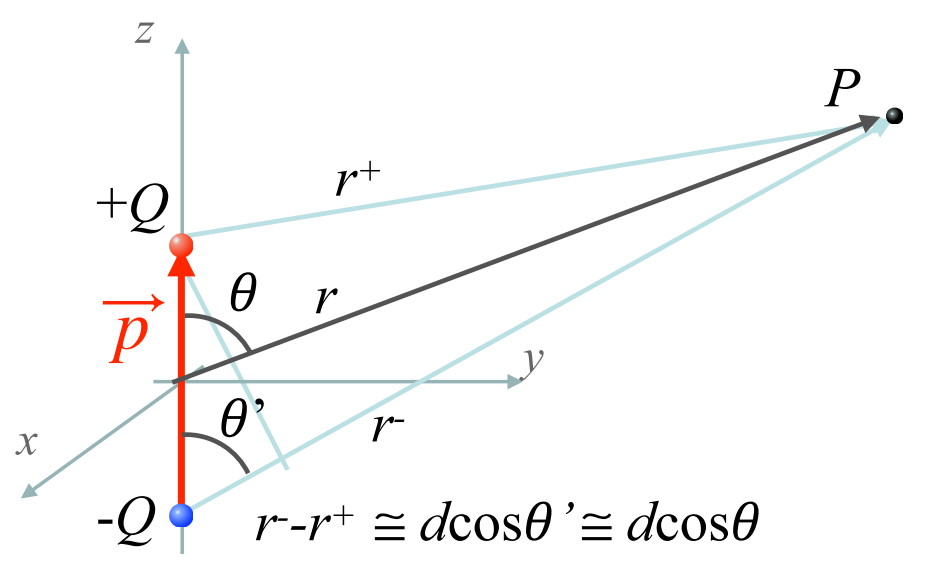
\includegraphics[scale=0.22]{img/Dipolo_elettrico}
\par\end{center}

Il dipolo elettrico viene matematicamente indicato con il \textbf{momento
di dipolo elettrico}: $\vec{p}=Q\vec{d}\quad\left(\text{in questo caso }=Qd\hat{k}\right)$
.

\paragraph*{Potenziale elettrostatico}

\[
V\left(\vec{r}\right)=\frac{1}{4\pi\varepsilon_{0}}\frac{+Q}{r^{+}}+\frac{1}{4\pi\varepsilon_{0}}\frac{-Q}{r^{-}}=\frac{Q}{4\pi\varepsilon_{0}}\left(\frac{1}{r^{+}}-\frac{1}{r^{-}}\right)
\]


\paragraph*{Potenziale elettrostatico $\left(r\gg d\right)$}

Nel caso in cui $r\gg d$ allora $r^{-}-r^{+}\cong d\cos\theta$ e
$r^{-}r^{+}\cong r^{2}$.

Allora $\vec{p}\cdot\vec{r}=pr\cos\theta=Qdr\cos\theta$ e il potenziale
risulta:

\[
V\left(\vec{r}\right)=\frac{1}{4\pi\varepsilon_{0}}\frac{\vec{p}\cdot\vec{r}}{r^{3}}
\]


\subsubsection*{Campo elettrico}

\[
\vec{E}\left(\vec{r}\right)=\frac{1}{4\pi\varepsilon_{0}r^{3}}\left[3\left(\vec{p}\cdot\vec{r}\right)\hat{r}-\vec{p}\right]
\]

Osservazioni:
\begin{itemize}
\item Il campo del dipolo elettrico descresce con la distanza come $\frac{1}{r^{3}}$.
\item In ogni punto il campo è la somma di una componenete radiale e di
una componenete parallela al vettore momento di dipolo.
\end{itemize}

\subsubsection*{Azioni meccaniche su un dipolo elettrico}

Calcoliamo il \textbf{momento della forza} esercitato da un campo
esterno $\vec{E}$ su un dipolo elettrico:

\[
\mathscr{M}=Fb=\left(QE\right)\left(d\sin\theta\right)=pE\sin\theta
\]

\[
\vec{\mathscr{M}}=\vec{p}\wedge\vec{E}
\]


\paragraph{Energia potenziale}

L'energia potenziale è descritta dalla formula $U=QV$ ma poichè in
un dipolo $V^{+}=-E\frac{d}{2}\cos\theta$ e $V^{-}=E\frac{d}{2}\cos\theta$
allora:

\[
U=QV^{+}+\left(-Q\right)V^{-}=-\left(Qd\right)E\cos\theta=-\vec{p}\cdot\vec{E}
\]

\begin{center}
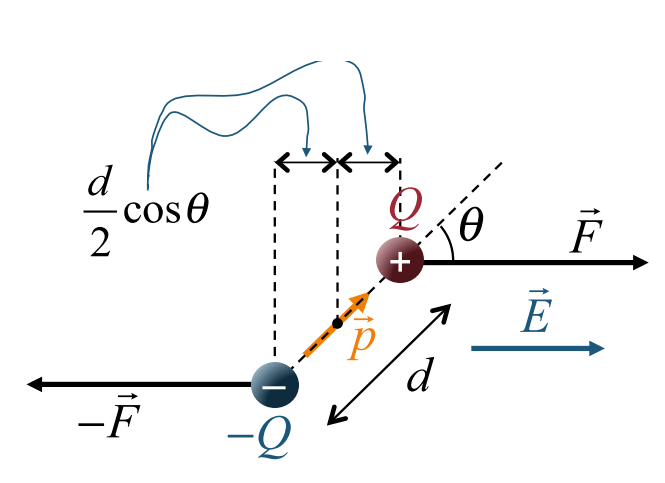
\includegraphics[scale=0.27]{img/Potenziale_di_un_dipolo_elettrico}
\par\end{center}

\pagebreak{}

\section{Elettrostatica dei conduttori}
\begin{center}
\begin{tabular}{|c|c|}
\hline 
\textbf{Materiali isolanti} & \textbf{Materiali conduttori}\tabularnewline
\hline 
\hline 
\multicolumn{1}{|c|}{Cariche localizzate, vincolate a muoversi} & Cariche libere di muoversi sul conduttore (almeno un\tabularnewline
all'interno delle molecole & elettrone per atomo è in grado di muoversi liberamente)\tabularnewline
\hline 
Un campo elettrico esterno non produce & In presenza di un campo esterno o di un eccesso di carica,\tabularnewline
movimento di cariche se non su piccola scala & le cariche si redistribuiscono sul conduttore\tabularnewline
\hline 
\end{tabular}
\par\end{center}

\subsection*{Conduttori in presenza di carica esterna}

In presenza di un campo elettrostatico esterno le cariche del conduttore
si spostano fino a raggiungere una nuova condizione di equilibrio
$\left(\Delta t\sim10^{9}\text{s}\right)$.
\begin{center}
Equilibrio $\Rightarrow$ cariche ferme $\Rightarrow$ forza nulla
$\Rightarrow$ campo elettrico complessivamente nullo
\par\end{center}

\begin{center}
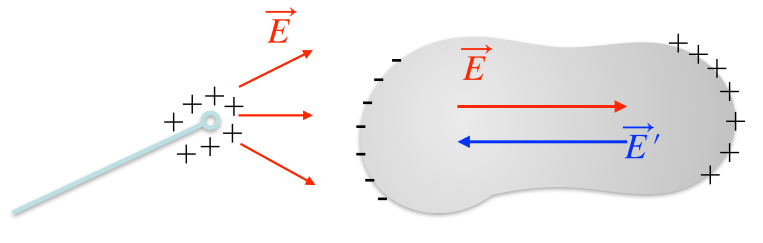
\includegraphics[scale=0.4]{img/Conduttori_in_presenza_di_carica_esterna}
\par\end{center}

Le cariche del conduttore si dispongono in modo da generare un campo
interno $\vec{E}'$ (indotto) che annulla il campo esterno $\vec{E}$:

\[
\vec{E}_{\text{condutt.}}=\vec{E}+\vec{E}'=0
\]

Dunque il campo elettrico interno ai conduttori è sempre nullo. Per
la legge di Gauss quindi:

\[
\Phi_{S}\left(\vec{E}\right)=\oiint_{S}\vec{E}\cdot\hat{n}\text{d}S=\frac{Q_{S}}{\varepsilon_{0}}=0\quad\Rightarrow\quad Q_{S}=\iiint\rho\text{d}\tau=0
\]

Osservazione: All'interno del conduttore \textbf{non ci sono cariche
in eccesso} (cariche positive e negative hanno uguale densità).

\subsubsection*{Carica superficiale di un consuttore}

Poichè abbiamo osservato che le cariche non sono all'interno ci viene
da pensare che esse di trovino all'esterno. In paricolare, la carica
in eccesso si dispone sulla superficie del conduttore in una configurazione
tale che il campo elettrico interno sia nullo.
\begin{center}
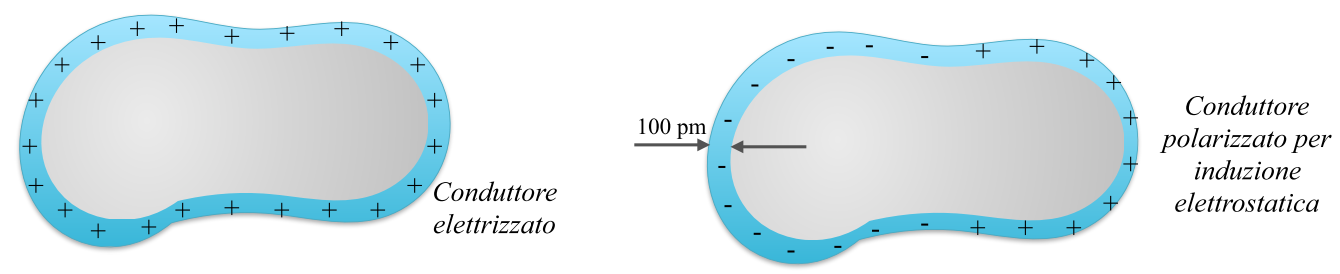
\includegraphics[scale=0.4]{img/Carica_superficiale_di_un_conduttore}
\par\end{center}

\begin{center}
\uline{Il campo elettrico è sempre normale alla superficie dei
conduttori}
\par\end{center}

In presenza di un conduttore, le linee di campo esterne vengono deviate
dalla presenza di addensamenti locali di carica sulla superficie del
conduttore. In conduttore deforma le linee di campo esterne in modo
che siano sempre perpendicolari alla sua superficie.

\[
\vec{E}=\frac{\sigma}{\varepsilon_{0}}\hat{n}
\]

\begin{center}
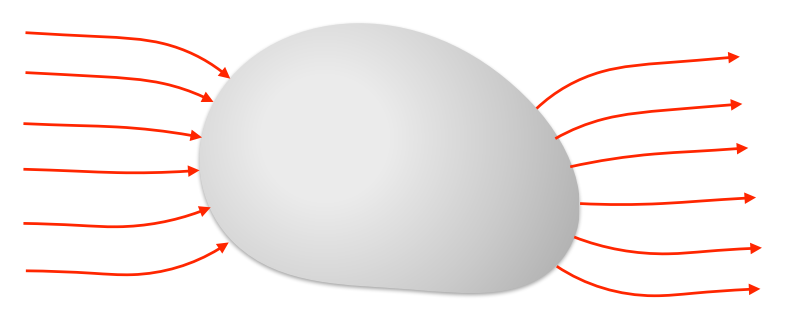
\includegraphics[scale=0.3]{img/Deformazione_delle_linee_di_campo_esterne_da_parte_di_un_conduttore}
\par\end{center}

\subsubsection*{Conduttori cavi}

Sulla superficie interna di un conduttore cavo\uline{ la carica
totale è nulla} e \uline{non si osservavo cariche localizzate}.
\begin{center}
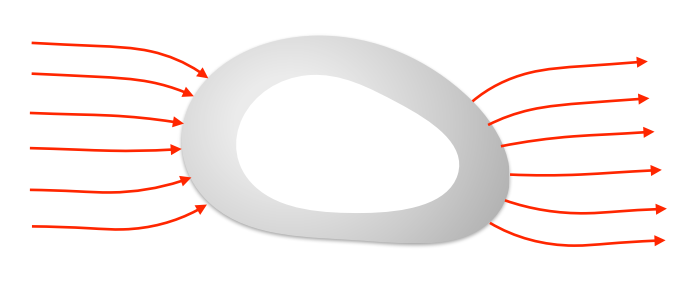
\includegraphics[scale=0.35]{img/Deformazione_delle_linee_di_campo_esterne_da_parte_di_un_conduttore_cavo}
\par\end{center}

Se un conduttore dotato di cavità viene esposto a un campo elettrico
esterno, il campo elettrico all’interno della cavità è comunque nullo
e non vi sono cariche elettriche indotte sulla superficie della cavità
stessa.

In altre parole il conduttore \textbf{scherma} l’interno della cavità
dai campi elettrici all’esterno (\textbf{gabbia di Faraday})

\paragraph*{Induzione completa}

Poniamo una carica puntiforme all’interno della cavità di un conduttore
neutro. La carica genera un campo con linee radiali che poi curvano
per diventare perpendicolari alla superficie interna.

Si parla cioè di induzione completa ovvero tutte le linee di forza
si chiudono sul conduttore.
\begin{center}
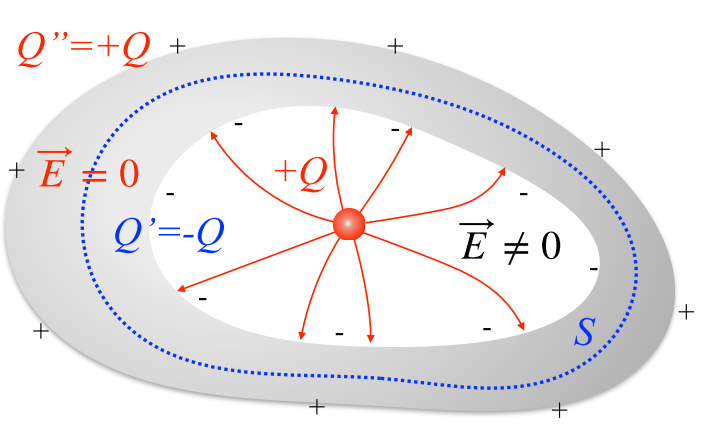
\includegraphics[scale=0.3]{img/Induzione_completa}
\par\end{center}

Osservazione: Un conduttore cavo trasferisce sulla propria superficie
esterna una carica uguale al valore complessivo delle cariche contenute
all’interno della cavità, quindi è possibile dall'esterno sapere se
all'interno è presente una carica.

\subsubsection*{Potenziale elettrostatico nei conduttori}

Tutti i punti del conduttore sono equipotenziali (la differenza di
potenziale tra due qualsiasi punti del conduttore è nulla):

\[
V_{A}-V_{B}=\int_{A}^{B}\vec{E}\cdot\text{d}\vec{l}=0\qquad\Rightarrow\quad V_{A}=V_{B}
\]


\subsection*{Capacità di un conduttore}

Definiamo capacità di un conduttore come il rapporto tra la carica
e il potenziale del conduttore:
\[
C=\frac{Q}{V}
\]

Nel S.I. la capacità si misura in Farad (F) e $\text{F}=\frac{\text{C}}{\text{V}}$
.
\begin{itemize}
\item La capacità quantifica l’attitudine di un conduttore ad accumulare
carica ad un dato potenziale.
\item La capacità dipende solo da forma e dimensione del conduttore e dal
mezzo che lo circonda.
\end{itemize}
\pagebreak{}

\subsection*{Condensatore}

La capacità di un conduttore aumenta se posto in vicinanza di un altro
conduttore:
\begin{center}
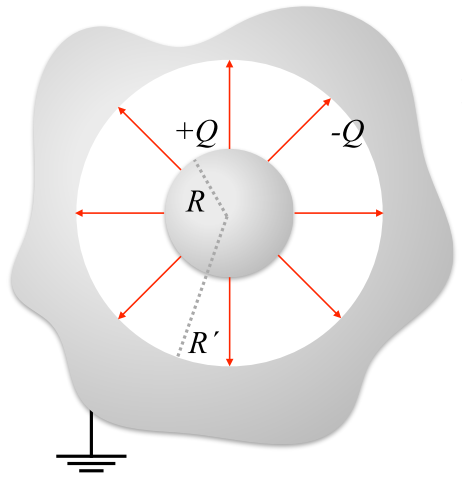
\includegraphics[scale=0.3]{img/Capacita_due_conduttori_vicini}
\par\end{center}

Notiamo come la capacità della sfera interna è maggiore alla capacità
della sfera isolata:

\[
V_{\text{int.}}=V\left(R\right)-V\left(R'\right)=\frac{Q}{4\pi\varepsilon_{0}}\int_{R}^{R'}\frac{\text{d}r}{r^{2}}=\frac{Q}{4\pi\varepsilon_{0}}\left(\frac{1}{R}-\frac{1}{R'}\right)\quad\Rightarrow\quad C_{\text{int.}}=\frac{Q}{V}=\frac{4\pi\varepsilon_{0}}{\left(\frac{1}{R}-\frac{1}{R'}\right)}>4\pi\varepsilon_{0}R=\frac{Q}{\frac{Q}{4\pi\varepsilon_{0}R}}=\frac{Q}{V}=C_{\text{isol.}}
\]

Il \textbf{condensatore} è un sistema formato da due conduttori carichi
per i quali si verifica induzione completa (tutte le linee di forza
uscenti da un conduttore incontrano l’altro conduttore). I due conduttori
sono le \textbf{armature} del condensatore, lo spazio interposto tra
le armature è l’\textbf{intercapedine}.
\begin{center}
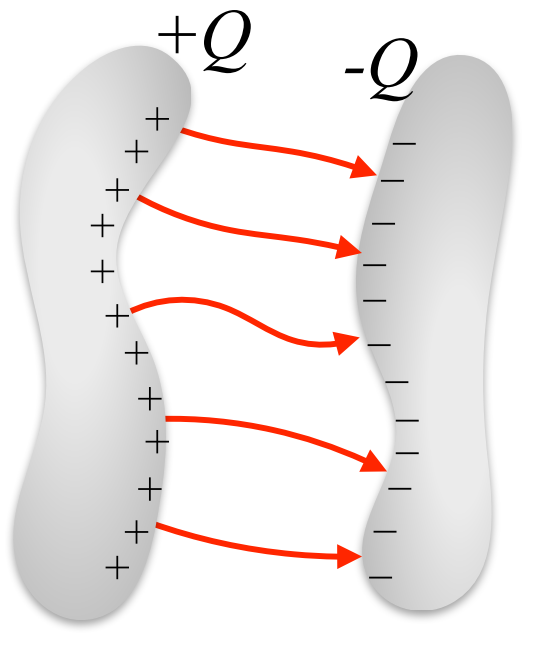
\includegraphics[scale=0.2]{img/Condensatore}
\par\end{center}

\[
C=\frac{Q}{\Delta V}
\]

\begin{center}
\begin{tabular}{|c|c|c|}
\hline 
Condensatore piano & Condensatore sferico & Condensatore cilindrico\tabularnewline
\hline 
\hline 
$C=\frac{\varepsilon_{0}S}{d}$ & $C=4\pi\varepsilon_{0}\left(\frac{R_{1}R_{2}}{R_{2}-R_{1}}\right)$ & $C=\frac{2\pi\varepsilon_{0}h}{\ln\frac{R_{2}}{R_{1}}}$\tabularnewline
\hline 
\end{tabular}
\par\end{center}

$\,$
\begin{center}
\textbf{Condensatori in parallelo}
\par\end{center}

\begin{center}
Nella connessione in parallelo gli elementi circuitati sono alla \uline{stessa
differenza di potenziale}.
\par\end{center}

\[
C_{\text{TOT}}=\Sigma C_{i}
\]

\begin{center}
\textbf{Condensatori in serie}
\par\end{center}

\begin{center}
Nella connessione in serie gli elementi circuitati hanno la \uline{stessa
carica}.
\par\end{center}

\[
\frac{1}{C_{\text{TOT}}}=\Sigma\frac{1}{C_{i}}
\]

\pagebreak{}

\subsection*{Energia elettrostatica di un sistema di cariche}

L'energia potenziale elettrostatica di una carica situata in un punto
dello spazio in cui è presente un potenziale $V$ vale:

\[
U=qV
\]

e rappresenta il lavoro che bisogna fare sulla carica $q$ per portarla
dall'infinito al punto in cui il potenziale vale $V$.

In un sistema di più cariche (ad esempio 3), per portare la prima
carica nella posizione non occorre fare lavoro, per portare la seconda
occorre fare un lavoro in contrapposizione al campo generato dalla
prima, per portare la terza occorre fare un lavoro in contrapposizione
al campo generato dalla prima e dalla seconda:

\[
U_{E}=U_{12}+U_{23}+U_{31}
\]

In generale:
\begin{center}
Sistema discreto
\par\end{center}

\[
U_{E}=\frac{1}{2}\sum_{i=1}^{n}q_{i}V_{i}=\frac{1}{2}\sum_{i=1}^{n}q_{i}\sum_{j\neq i}^{n}\frac{q_{j}}{4\pi\varepsilon_{0}r_{ij}}
\]

\begin{center}
Sistema continuo
\par\end{center}

\[
U_{E}=\frac{1}{2}\int_{\tau}\rho V\text{d}\tau
\]

In alternativa utilizzando la legge di Gauss in forma locale: $\rho=\varepsilon_{0}\vec{\nabla}\cdot\vec{E}$
possiamo ridefinire la formula precedente mediante il concetto di
\textbf{densità di energia} del campo elettrostatico:

\[
u_{E}=\frac{1}{2}\varepsilon_{0}E^{2}
\]

e dunque

\[
U_{E}=\underset{\text{spazio}}{\int}u_{E}\text{d}\tau
\]


\subsection*{Energia di un condensatore}

Il lavoro infinitesimo per portare una carica $+\text{d}q$ dall'armatura
caricata negativamente a quella caricata positivamente è:

\[
\text{d}\mathscr{L}=\text{d}q\Delta V_{q}=\text{d}q\frac{q}{C}
\]

Il lavoro complessivo per caricare completamente il condensatore dalla
carica 0 alla carica Q:

\[
\mathscr{L}=\int_{0}^{Q}\text{d}\mathscr{L}=\frac{1}{2}\frac{Q^{2}}{C}
\]

L’energia elettrostatica accumulata in un condensatore è

\[
U_{E}\;=\;\frac{1}{2}\frac{Q^{2}}{C}\;=\;\frac{1}{2}Q\Delta V\;=\;\frac{1}{2}C\Delta V^{2}\;=\;\int_{\tau}u_{E}\text{d}\tau
\]

\pagebreak{}

\subsection*{Forza tra le armature di un condensatore}

Le armature di un condensatore hanno cariche opposte e dunque si attraggono. 
\begin{center}
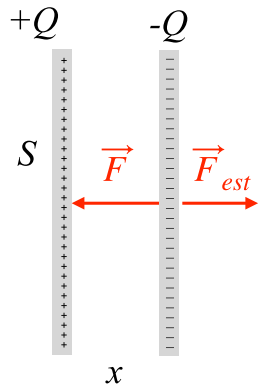
\includegraphics[scale=0.35]{img/Forza_tra_le_armature_di_un_condensatore}
\par\end{center}

Colcoliamo la forza tra le armature partendo dall'energia

\[
U_{E}=\frac{1}{2}\frac{Q^{2}x}{\varepsilon_{0}S}\Rightarrow\text{d}U_{E}=\frac{1}{2}\frac{Q^{2}\text{d}x}{\varepsilon_{0}S}=\delta\mathscr{L}_{\text{est}}=F_{\text{est}}\text{d}x
\]

quindi:

\[
\vec{F}=-\vec{F}_{\text{est}}=-\frac{Q^{2}}{2\varepsilon_{0}S}\hat{n}
\]

Si definisce \textbf{pressione elettrostatica} :

\[
p=\frac{F}{S}=\frac{Q^{2}}{2\varepsilon_{0}S^{2}}=\frac{\sigma^{2}}{2\varepsilon_{0}}
\]

\pagebreak{}

\subsection*{Condensatori con dielettrici}
\begin{center}
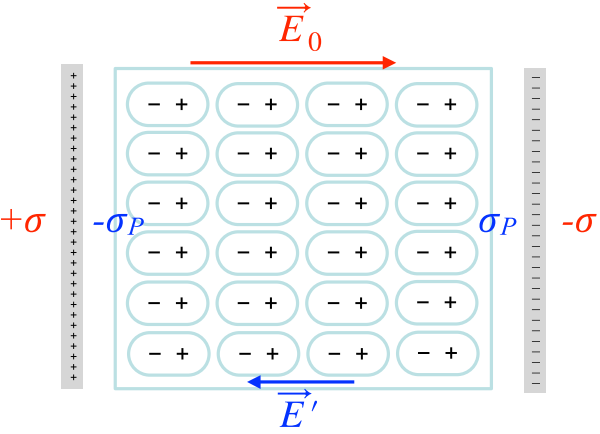
\includegraphics[scale=0.35]{img/Condensatore_con_dielettrici}
\par\end{center}

Se riempiamo con materiale isolante l'intercapedine di un condensatore,
le cariche del dielettrico non si muovono, però a livello microscopico
sulle superfici del dielettrico a contatto con le armature del condensatore
si osserva un eccesso di carica $\sigma_{P}$ (\textbf{carica di polarizzazione}).
Le cariche di polarizzazione creano un campo elettrico opposto al
campo del condensatore.

\uline{Il campo elettrico totale} (e di conseguenza la differenza
di potenziale) \uline{diminuisce} mentre\uline{ la capacità
del condensatore aumenta}.
\begin{center}
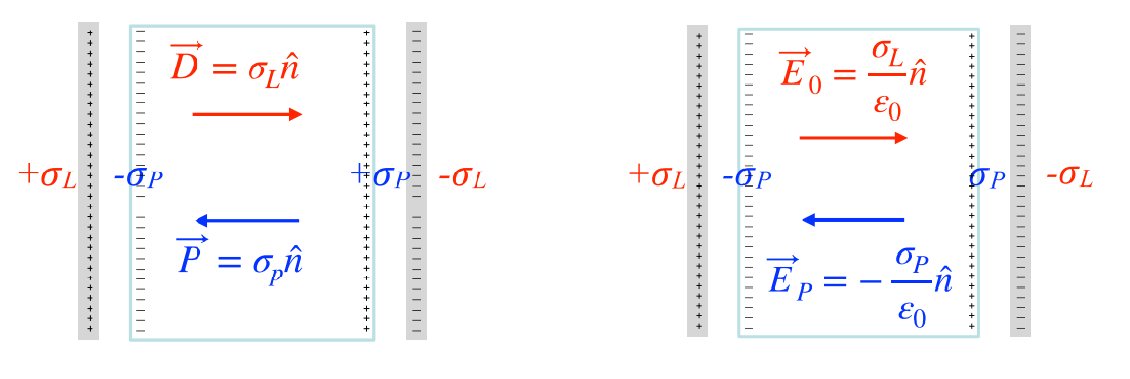
\includegraphics[scale=0.45]{img/Elettrostatica_dei_dielettrici}
\par\end{center}

Ogni singola molecola si allineerà rispetto al momento delle forze
a cui è soggetta: $\vec{\mathscr{M}}=\vec{p}\wedge\vec{E}_{0}$. 

Definiamo il \textbf{momento di dipolo medio }con il simbolo $\left\langle \vec{p}\right\rangle $.

Sia $n=\frac{N}{\Delta\tau}$ il numero di atomi/molecole per unità
di volume, si definisce \textbf{vettore polarizzazione} $\vec{P}=n\left\langle \vec{p}\right\rangle $.

Il modulo del vettore polarizzazione è la \textbf{densità di carica
di polarizzazione} $\left|\vec{P}\right|=\sigma_{P}$.

Si definisce \textbf{vettore spostamento elettrico} $\vec{D}=\sigma_{L}\hat{n}$

Oss: Il un dielettrico isotropo (è uguale in tutto lo spazio) e omogeneo
(la materia è distribuita nello spazio allo stesso modo):
\begin{itemize}
\item le cariche di polarizzazione sono distribuite solo superficialmente
\item i vettori campo elettrico, polarizzazione e spostamento elettrico
sono paralleli
\item si definiscono le due quantità adimensionali \textbf{suscettività
elettrica} $\chi\;\left(\chi>0\right)$ e \textbf{costante dielettrica
relativa }$\varepsilon_{R}\;\left(\varepsilon_{R}\geq1\right)$ legate
dalla relazione:
\end{itemize}
\[
\chi=\varepsilon_{R}-1
\]


\paragraph*{Riformulazione di vettore polarizzazione e vettore spostamento elettrico}

\[
\vec{P}=\varepsilon_{0}\chi\vec{E}=\varepsilon_{0}\left(\varepsilon_{R}-1\right)\vec{E}
\]

\[
\vec{D}=\varepsilon_{0}\vec{E}+\vec{P}=\varepsilon_{0}\vec{E}+\varepsilon_{0}\left(\varepsilon_{R}-1\right)\vec{E}=\varepsilon_{0}\varepsilon_{R}\vec{E}
\]


\paragraph*{Riformulazione legge di Gauss in funzione delle cariche libere}

\[
\vec{\nabla}\cdot\vec{D}=\rho_{L}\qquad\qquad\oiint\vec{D}\cdot\hat{n}\text{d}S=Q_{L}
\]


\paragraph*{Formule condensatore con dielettrico}
\begin{itemize}
\item Campo elettrico:
\end{itemize}
\[
\vec{E}=\frac{\vec{D}}{\varepsilon_{0}\varepsilon_{R}}=\frac{\sigma_{L}\hat{n}}{\varepsilon_{0}\varepsilon_{R}}=\frac{\vec{E}_{0}}{\varepsilon_{R}}\qquad\vec{E}_{0}\text{ è il campo elettrico con condensatore vuoto}
\]

\begin{itemize}
\item Potenziale elettrico:
\end{itemize}
\[
\Delta V=\frac{\Delta V_{0}}{\varepsilon_{R}}\qquad\vec{V}_{0}\text{ è il potenziale elettrico con condensatore vuoto}
\]

\begin{itemize}
\item Capacità condensatore con dielettrico:
\end{itemize}
\[
C=\frac{Q}{\Delta V}=\varepsilon_{R}\frac{Q}{\Delta V_{0}}=\varepsilon_{R}C_{0}\qquad C_{0}\text{ è la capacità con condensatore vuoto}
\]

\begin{itemize}
\item Capacità condensatore piano con dielettrico
\end{itemize}
\[
C=\frac{\varepsilon_{0}\varepsilon_{R}S}{d}
\]

\pagebreak{}

\section{Correnti elettriche}

\subsection*{Modello di Drude-Lorentz}

Se tramite un generatore si pone una differenza di potenziale (d.d.p.)
tra due punti del conduttore gli elettroni di conduzione si mettono
in moto ed il conduttore risulta percorso da una corrente elettrica.

Se la d.d.p. è costante ci si aspetta che il moto degli elettroni
sia uniformemente accelerato. Sperimentalmente però si trova che la
velocità media degli elettroni è proporzionale al campo mentre l'accelerazione
no: $\left\langle \vec{v}_{e}\right\rangle \propto\vec{E}$.

Questo perchè gli elettroni nel loro moto urtano contro i protoni
cedendo energia, dunque rallentano e aumentano l'energia vibrazionale
e conseguentemente la temperatura.

La velocità media con cui si muovono gli elettroni è detta velocità
di deriva:

\[
\vec{v}_{e}=\vec{a}_{e}t=\frac{q_{e}}{m_{e}}\vec{E}t\quad\Rightarrow\quad\vec{v}_{d}=\left\langle \vec{v}_{e}\right\rangle =\frac{q_{e}}{m_{e}}\vec{E}\left\langle t\right\rangle 
\]

Con $\left\langle t\right\rangle $ il tempo medio che intercorre
tra due urti.

Gli elettroni possiedono anche una velocità dovuta all’agitazione
termica, ma si può dimostrare che essa ha valore medio nullo (perché
casuale in ogni direzione).

\subsection*{Intensità di corrente}

Data una sezione $S$ di un conduttore all'interno del quale è mantenuta
una differenza di potenziale, definiamo l'\textbf{intensità di corrente}
elettrica come la quantità di carica che attraversa il conduttore
per unità di tempo:

\[
i=\lim_{\Delta t\rightarrow0}\frac{\Delta q}{\Delta t}=\frac{\text{d}q}{\text{d}t}
\]

\begin{center}
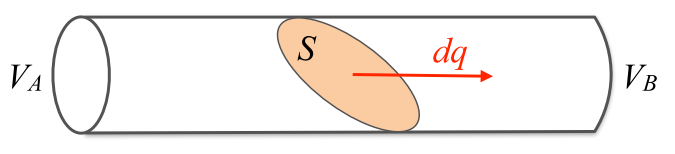
\includegraphics[scale=0.35]{img/Intensita_di_corrente}
\par\end{center}

Nel S.I. l'unità di misura della corrente è l'Ampere ($\text{A}=\frac{\text{C}}{\text{s}}$).

Dal punto di vista sperimentale, in elettromagnetismo, il moto di
una carica positiva è equivalente al moto di una carica negativa che
procede in verso opposto. La convenzione impone il verso positivo
delle correnti quello in cui si muovono i portatori di carica positivi.

\subsection*{Vettore densità di corrente elettrica}

Definiamo il vettore densità di corrente elettrica come la corrente
che passa attraverso l'unità di superificie $\text{d}S$ ed ha verso
della velocià di deriva:

\[
\vec{j}=nq_{e}\vec{v}_{d}
\]

\begin{center}
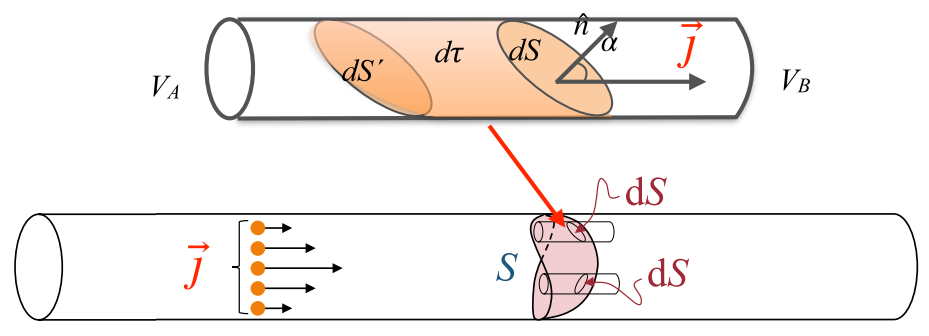
\includegraphics[scale=0.35]{img/Vettore_densita_di_corrente}
\par\end{center}

Il flusso della densità di corrente elettrica, attraverso una superficie
chiusa insterna al conduttore, rappresenta la corrente elettrica che
attraversa tale superficie:

\[
\text{d}i=\left(\frac{\text{d}q}{\text{d}t}\right)_{\text{d}S}=\vec{j}\cdot\hat{n}\text{d}S\quad\Rightarrow\quad i=\Phi_{S}\left(\vec{j}\right)=\oiint_{S}\vec{j}\cdot\hat{n}\text{d}S
\]

\pagebreak{}

\subsection*{Equazione di continuità}

Per il teorema della divergenza possiamo riscrivere $i=\oiint_{S}\vec{j}\cdot\hat{n}\text{d}S=\iiint_{\tau_{S}}\vec{\nabla}\cdot\vec{j}\text{d}\tau$

Possiamo considerare la corrente uscente $i_{\text{uscente}}=-\frac{\text{d}q}{\text{d}t}=-\frac{\partial}{\partial t}\iiint_{\tau_{S}}\rho\text{d}\tau=-\iiint_{\tau_{S}}\frac{\partial\rho}{\partial t}\text{d}\tau$
data $q=\iiint_{\tau_{S}}\rho\text{d}\tau$

Considerando che la corrente $i$ e quella uscente $i_{\text{uscente}}$
sono in modulo uguali e che il dominio di integrazione $\tau_{S}$
è lo stesso per le due espressioni si ricava la formula:

\[
\vec{\nabla}\cdot\vec{j}=-\frac{\partial\rho}{\partial t}
\]

Cioè la divergenza del vettore di densità bilancia la variazione di
carica.

\subsection*{Prima legge di Ohm}

La costante di proporzionalità tra l'intensità di corrente e la differenza
di potenziale è la \textbf{resistenza elettrica}.

\[
\Delta V=Ri
\]

La resistenza nel S.I. si misura in Ohm ($\Omega=\frac{\text{V}}{A}$).

\subsection*{Seconda legge di Ohm}

La resistenza di un conduttore omogeneo, filiforme di lunghezza $l$
e sezione $S$ vale:

\[
R=\rho_{R}\frac{l}{S}
\]

dove $\rho_{R}$ è detta \textbf{resistività elettrica} e dipende
dalla natura del materiale.

Chiamiamo invece \textbf{conduttività elettrica} il rapporto $\sigma_{C}=\frac{1}{\rho_{R}}$.

\subsection*{Leggi di Ohm in forma locale}

Per la definizione di differenziale di corrente elettrica si ha che
$\text{d}i=j\text{d}S$.

Per le due leggi di Ohm si ha che $\text{d}V=R\text{d}i=\rho_{R}\frac{\text{d}l}{\text{d}S}\text{d}i=\rho_{R}j\text{d}l$.

Infine dalla definizione di differenziale di potenziale $\text{d}V=E\text{d}l$
di può ricavare che

\[
\vec{E}=\rho_{R}\vec{j}\qquad\equiv\qquad\vec{j}=\sigma_{C}\vec{E}
\]


\subsection*{Resistenza}
\begin{center}
\textbf{Resistenze in serie}
\par\end{center}

\begin{center}
Nella connessione in serie gli elementi circuitati sono attraversati
dalla \uline{stessa corrente}.
\par\end{center}

\[
R_{\text{TOT}}=\Sigma R_{i}
\]

\begin{center}
\textbf{Resistenze in parallelo}
\par\end{center}

\begin{center}
Nella connessione in parallelo gli elementi circuitati sono alla \uline{stessa
differenza di potenziale}.
\par\end{center}

\[
\frac{1}{R_{\text{TOT}}}=\Sigma\frac{1}{R_{i}}
\]


\subsection*{Effetto Joule}

L'effetto Joule consiste nella dissipazione della potenza dovuta agli
urti degli elettroni con gli atomi di un conduttore, i quali aumentano
la propria energia vibrazionale e producono come risultato un aumento
della temperatura. Calcoliamo tale potenza:

$\,$

Quando una corrente $i$ scorre attraverso un conduttore filiforme,
la carica che attraversa una sezione $S$ in un tempo $\text{d}t$
è $\text{d}q=i\text{d}t$.

Il lavoro compiuto dal campo elettrico nello spostamento di una carica
$q$ nell'intervallo $\text{d}t$ è:

\[
\delta\mathscr{L}=\text{d}U=\Delta V\text{d}q=\left(Ri\right)i\text{d}t=Ri^{2}\text{d}t
\]

Definiamo la\textbf{ potenza}:

\[
P=\frac{\text{d}U}{\text{d}t}=Ri^{2}=i\Delta V=\frac{\Delta V^{2}}{R}
\]

La potenza nel S.I. si misura in Watt ($\text{W}=\frac{\text{J}}{s}$).

\subsection*{Effetto Joule in forma locale}

Relazione locale che esprime la potenza applicata sugli $N$ elettroni
contenuti in un volume $\text{d}\tau$:

\[
\frac{\text{d}P}{\text{d}\tau}=\frac{\delta\mathscr{L}}{\text{d}\tau\text{d}t}=\vec{E}\cdot\vec{j}
\]


\subsection*{Superconduttori}

Alcuni metalli o leghe, al di sotto di una temperatura critica $T_{c}$
prossima allo zero assoluto mostrano una resistività nulla. In tali
condizioni di superconduttività, le correnti circolano senza dissipazione
di energia e i superconduttori non si riscaldano, anche con correnti
molto intense.

\subsection*{Generatore di forza elettromotrice}
\begin{center}
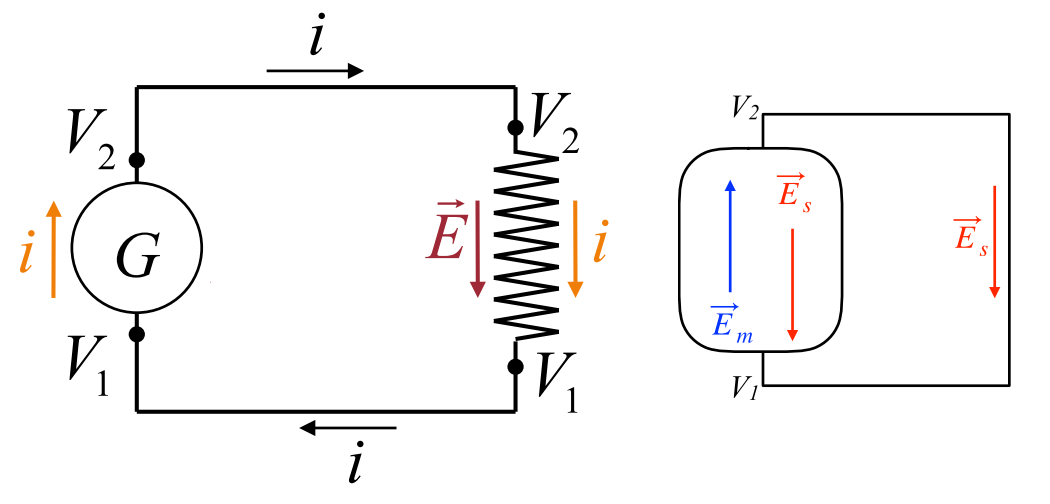
\includegraphics[scale=0.3]{img/Generatore_di_forza_elettromotricePNG}
\par\end{center}

Tra di due capi del generatore si deve avere una differenza di potenziale
dato che nel circuito è presente una corrente.

All'interno del generatore si ha il campo elettromotore $\vec{E}_{m}$
(non conservativo). La\textbf{ forza elettromotrice} si calcola:

\[
\mathscr{E}=\oint\vec{E}_{m}\cdot\text{d}\vec{l}=-\oint\vec{E}_{S}\cdot\text{d}\vec{l}=\Delta V
\]

\begin{center}
\begin{tabular}{|c|c|}
\hline 
\textbf{Generatori ideali} & \textbf{Generatori reali}\tabularnewline
\hline 
\hline 
La tensione ai capi del generatore si mantiene costante & La tensione ai capi del generatore presenta una caduta ohmica\tabularnewline
 & (Occorre considerare una resistenza interna al generatore)\tabularnewline
\hline 
\multicolumn{1}{c}{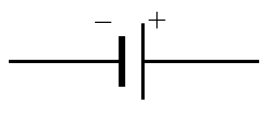
\includegraphics[scale=0.23]{img/Generatore_ideale}} & \multicolumn{1}{c}{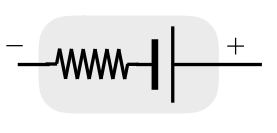
\includegraphics[scale=0.25]{img/Generatore_reale}}\tabularnewline
\end{tabular}
\par\end{center}

\pagebreak{}

\subsection*{Prima legge di Kirchoff}

In qualunque nodo di un circuito la corrente totale entrante è uguale
alla corrente totale uscente:

\[
\sum_{\text{nodo}}i_{k}=\sum_{\text{entranti}}i_{k}-\sum_{\text{uscenti}}i_{k}=0
\]


\subsection*{Seconda legge di Kirchoff}

Su qualunque maglia di un circuito la caduta di potenziale è uguale
alla somma delle tensioni erogate dai generatori:

\[
\sum_{k}\mathscr{E}_{k}=R_{\text{tot}}i=\Delta V
\]


\subsection*{Circuiti RC in regime transitorio}

Si tratta di circuiti (ideali) formati da una resistenza, un condensatore
e da un generatore di forza elettromotrice.
\begin{center}
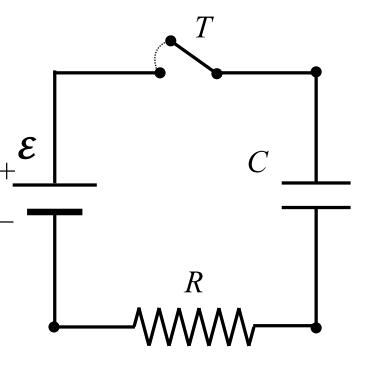
\includegraphics[scale=0.35]{img/Circuito_RC}
\par\end{center}

\subsubsection*{Carica di un condensatore}

Nel caso si vada a chiudere l'interruttore si avrà che ai capi della
resistenza la differenza di potenziale è $\Delta V_{R}\left(t\right)=Ri\left(t\right)$
mentre ai capi del condensatore $\Delta V_{C}\left(t\right)=\frac{Q\left(t\right)}{C}$.
Applicando la legge delle maglie:
\begin{center}
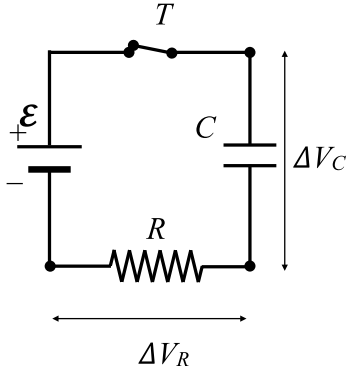
\includegraphics[scale=0.3]{img/Carica_condensatore}
\par\end{center}

\[
\mathscr{E}=\Delta V_{R}\left(t\right)+\Delta V_{C}\left(t\right)=Ri\left(t\right)+\frac{Q\left(t\right)}{C}=\text{derivando rispetto a \ensuremath{t}}\Rightarrow0=R\frac{\text{d}i}{\text{d}t}+\frac{1}{C}\frac{\text{d}Q}{\text{d}t}=R\frac{\text{d}i}{\text{d}t}+\frac{i}{C}\Rightarrow
\]

\[
\Rightarrow\frac{\text{d}i}{i}=-\frac{\text{d}t}{RC}\Rightarrow\int_{i\left(0\right)}^{i\left(t\right)}\frac{\text{d}i'}{i'}=-\frac{1}{RC}\int_{0}^{t}\text{d}t'\Rightarrow\ln\left(\frac{i\left(t\right)}{i\left(0\right)}\right)=-\frac{t}{RC}\Rightarrow i\left(t\right)=i\left(0\right)e^{-\frac{t}{RC}}\Rightarrow
\]

\[
\text{Nell'istante iniziale }\mathscr{E}=Ri\left(0\right)+\frac{\overset{0}{\overbrace{Q\left(0\right)}}}{C}=Ri\left(0\right)\Rightarrow i\left(0\right)=\frac{\mathscr{E}}{R}
\]

\[
i\left(t\right)=\frac{\mathscr{E}}{R}e^{-\frac{t}{\tau}}\qquad\tau=RC
\]

\[
\Delta V_{R}\left(t\right)=Ri\left(t\right)=\mathscr{E}e^{-\frac{t}{\tau}}\qquad\tau=RC
\]

\[
Q\left(t\right)=\int i\left(t\right)\text{d}t=\mathscr{E}C\left(1-e^{-\frac{t}{\tau}}\right)\qquad\tau=RC
\]

\[
\Delta V_{C}\left(t\right)=\frac{Q\left(t\right)}{C}=\mathscr{E}\left(1-e^{-\frac{t}{\tau}}\right)\qquad\tau=RC
\]


\subsubsection*{Scarica di un condensatore}

L'equazione alle maglie alla chiusura dell'interrutore è:

\[
0=\mathscr{E}=\Delta V_{R}\left(t\right)+\Delta V_{C}\left(t\right)=Ri\left(t\right)+\frac{Q\left(t\right)}{C}=R\frac{\text{d}Q}{\text{d}t}+\frac{Q}{C}\Rightarrow\frac{\text{d}Q}{Q}=-\frac{\text{d}t}{RC}\Rightarrow
\]

\[
\Rightarrow\int_{Q\left(0\right)}^{Q\left(t\right)}\frac{\text{d}Q'}{Q'}=-\frac{1}{RC}\int_{0}^{t}\text{d}t'\Rightarrow\ln\left(\frac{Q\left(t\right)}{Q\left(0\right)}\right)=-\frac{t}{RC}\Rightarrow Q\left(t\right)=Q\left(0\right)e^{-\frac{t}{RC}}
\]

\begin{center}
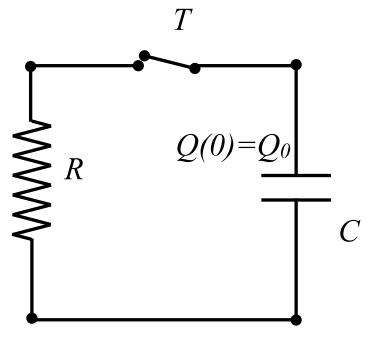
\includegraphics[scale=0.3]{img/Scarica_condensatore}
\par\end{center}

\[
Q\left(t\right)=Q_{0}e^{-\frac{t}{\tau}}\qquad\tau=RC
\]

\[
i\left(t\right)=\frac{\text{d}Q}{\text{d}t}=-\frac{Q_{0}}{\tau}e^{-\frac{t}{\tau}}=-\frac{V_{C}}{R}e^{-\frac{t}{\tau}}\qquad\tau=RC
\]

\[
U_{R}=\int_{0}^{\infty}P_{R}dt=\int_{0}^{\infty}Ri^{2}dt=\frac{1}{2}CV_{C}^{2}=U_{C}
\]

\begin{center}
Cioè l'energia che era inizialmente accumulata nel condensatore viene
interamente dissipata sulla resistenza
\par\end{center}

\pagebreak{}

\section{Campi Magnetici Stazionari}

Si introduce un campo vettoriale $\vec{B}$ detto \textbf{campo magnetico}
o campo induzione magnetica le cui linee di forza entrano nel polo
sud ed escono dal polo nord di un ipotetico ago magnetico e dunque
è tangente alla sua direzione.
\begin{center}
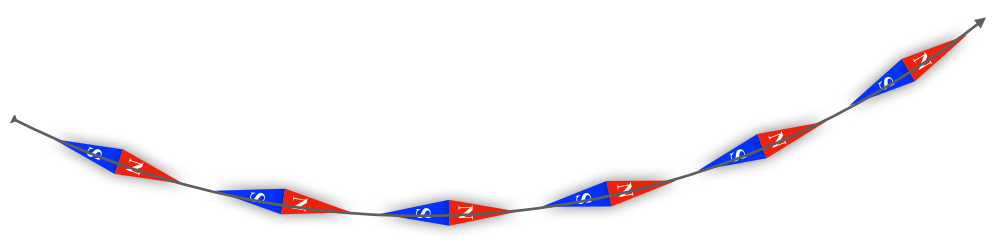
\includegraphics[scale=0.4]{img/Aghi_magnetici}
\par\end{center}

Il polo nord magnetico coincide con il polo sud geografico.

Nel S.I. il campo magnetico si misura in Testa $\text{T}=\frac{Vs}{m^{2}}$

Un campo magnetico è generato da cariche in movimento e cioè da correnti.
\begin{center}
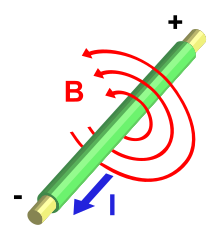
\includegraphics[scale=0.45]{img/Linee_di_campo_magnetico_rispetto_ad_una_corrente}
\par\end{center}

Il campo magnetico è solenoidale $\left(\vec{\nabla}\cdot\vec{B}=0\right)$
cioè non è conservativo (perchè vedremo che dipende dalla velocità
delle cariche elettriche).

\subsection*{Seconda legge di Laplace}

Un tratto di filo $\text{d}\vec{l}$ percorso da una corrente $i$
ed immerso in un campo di induzione magnetica $\vec{B}$ subisce una
forza descritta da:

\[
\text{d}\vec{F}=i\text{d}\vec{l}\wedge\vec{B}
\]

\begin{center}
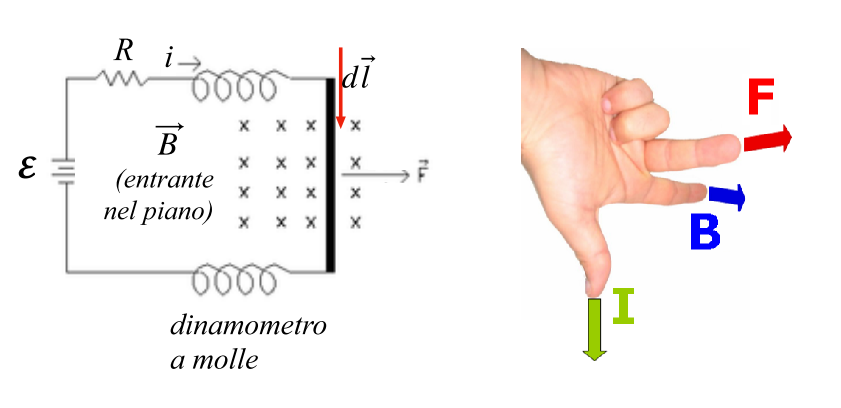
\includegraphics[scale=0.4]{img/Seconda_legge_di_laplace}
\par\end{center}

\subsection*{Forza di Lorentz}

Una carica puntiforme $q$ in moto con velocità $\vec{v}$ in presenza
di un campo di induzione magnetica $\vec{B}$ subisce una forza pari
a:

\[
\vec{F}_{\text{Lorentz}}=q\vec{v}\wedge\vec{B}
\]

La forza di Lorentz dipende dalla velocità e dunque non è conservativa.

In presenza di un campo elettrico che un campo magnetico la forza
di Lorentz si scrive:

\[
\vec{F}_{\text{Lorentz}}=q\vec{E}+q\vec{v}\wedge\vec{B}
\]


\subsubsection*{Moto di cariche in campi magnetici}

Studiamo il moto di una carica $q$ che si muove con velocità costante
$\vec{v}$, perpendicolare ad un campo magnetico uniforme $\vec{B}$:
\begin{center}
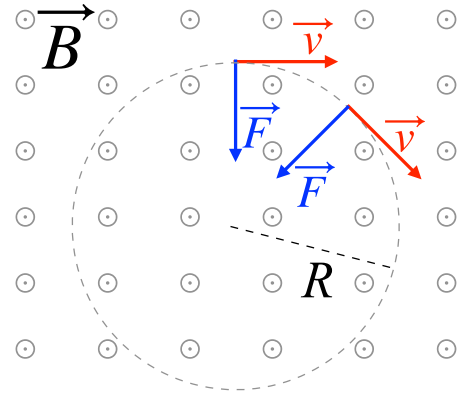
\includegraphics[scale=0.3]{img/Moto_cariche_in_campo_magnetico_con_velocita_ortogonale_al_campo}
\par\end{center}

\[
F_{\text{centripeta}}=m\frac{v^{2}}{R}=qvB=F_{\text{Lorentz}}
\]

\[
R=\frac{mv}{qB}
\]

\[
T=\frac{2\pi R}{v}=2\pi\frac{m}{qB}
\]

\[
\omega=\frac{2\pi}{T}=\frac{qB}{m}
\]


\subsubsection*{Effetto Hall}

Consideriamo un conduttore metallico a sezione rettangolare ($d\times h$)
percorso da corrente $i$. Poniamo il sistema in un campo magnetico
uniforme
\begin{center}
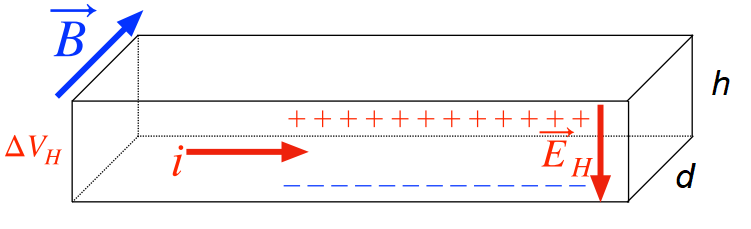
\includegraphics[scale=0.4]{img/Effetto_Hall}
\par\end{center}

\begin{center}
\textbf{Campo di Hall}
\par\end{center}

\begin{center}
\[
\vec{F}_{\text{Lorentz}}=qv_{d}B=qE_{H}=\vec{F}_{\text{elettrostatica}}
\]
\par\end{center}

\begin{center}
\textbf{Potenziale di Hall}
\par\end{center}

\[
\Delta V_{H}=E_{H}h=v_{d}Bh=\frac{i}{nqd}B=R_{H}\frac{iB}{d}
\]

dove $R_{H}=\frac{1}{nq}\left(\sim10^{-11}\frac{m^{3}}{C}\right)$
è la \textbf{costante di Hall}. 

\pagebreak{}

\subsection*{Circuito in un campo magnetico}

La forza totale esercitata su un tratto del circuito $\text{d}\vec{l}$
percorso da una corrente $i$ da parte di un campo magnetico $\vec{B}$
ricavata dalla seconda legge di Laplace è:

\[
\vec{F}=i\oint\text{d}\vec{l}\wedge\vec{B}
\]

Il momento delle forze è:

\[
\vec{\mathscr{M}}=\oint\vec{r}\wedge\text{d}\vec{F}=i\oint\vec{r}\wedge\left(\text{d}\vec{l}\wedge\vec{B}\right)
\]

dove $r$ è la distanza di un punto dall'asse di rotazione.

Considerando una spira rettangolare immersa in un campo magnetico
uniforme essa non translerà poichè la risultante delle forze a cui
è sottoposta è nulla, ma ruoterà perchè il momento delle forze non
è nullo.

In generale per una spira di qualsiasi forma \uline{la risutante
dell forze sarà sempre nulla} mentre si ha che il \textbf{momento
magnetico della spira} vale
\[
\vec{m}=iS\hat{n}
\]

e il momento delle forze si può calcolare come

\[
\vec{\mathscr{M}}=\vec{m}\wedge\vec{B}
\]


\subsubsection*{Teorema di equivalenza di Ampère}

Una spira percorsa da corrente e immersa in un campo magnetico si
comporta come un dipolo magnetico elementare (ago magnetico) di momento
$\vec{m}=iS\hat{n}$, perpendicolare al piano della spira e orientato
con la regola della mano destra.
\begin{center}
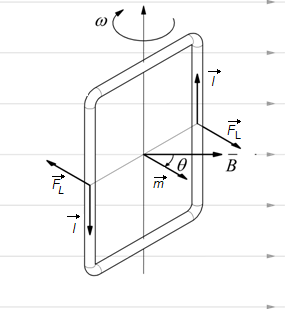
\includegraphics[scale=0.6]{img/Teorema_di_equivalenza_di_Ampere}
\par\end{center}

\subsubsection*{Piccole oscillazioni di una spira}

Consideriamo una spira il cui momento magnetico forma con il campo
magnetico un angolo $\theta\approx0$.

La spira avrà un momento di inerzia $I$ e si comporterà come un pendolo
fisico.

Conoscendo la corrente e momento di inerzia della spira, abbiamo un
metodo per misurare l’intensità del campo $B$ a partire dalla misura
del periodo di oscillazione:

\[
B=\frac{I}{iS}\left(\frac{2\pi}{T}\right)^{2}
\]


\subsubsection*{Energia di una spira}

\[
\text{d}\mathscr{L}=\mathscr{M}\text{d}\theta=mB\sin\theta\text{d}\theta\Rightarrow\mathscr{L}=\int mB\sin\theta\text{d}\theta=-mB\cos\theta=-\vec{m}\cdot\vec{B}
\]

\[
U_{M}=-\vec{m}\cdot\vec{B}
\]


\subsection*{Galvanometro}

Il galvanometro è uno strumento utilizzato per misurare piccole intensità
di corrente. Il momento delle forze magnetiche $\mathscr{M}_{M}=-iSB\sin\theta\sim-iSB$
sulla spira è bilanciato dal momento delle forze elastiche $\mathscr{M}_{\text{molla}}=-k\alpha$.
La misura della corrente è data da:

\[
i=\frac{k\alpha}{SB}
\]

\begin{center}
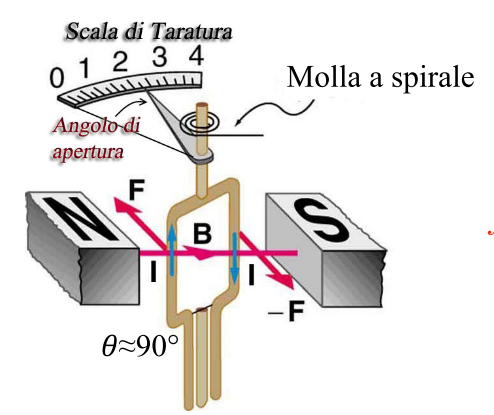
\includegraphics[scale=0.35]{img/Galvanometro}
\par\end{center}

\subsection*{Prima legge di Laplace}

Evidenze sperimentali mostrano che i fili percorsi da corrente generano
campi magnetici: in particolare un filo infinitesimo $\text{d}\vec{l}$
percorso da una corrente $i$ genera un campo magnetico infinitesimo
a distanza $r$ pari a: 

\[
\text{d}\vec{B}=\frac{\mu_{0}}{4\pi}\frac{i\text{d}\vec{l}\wedge\hat{r}}{r^{2}}=\frac{\mu_{0}}{4\pi}\frac{i\text{d}\vec{l}\wedge\vec{r}}{r^{3}}
\]

dove la costante $\mu_{0}$è detta \textbf{permeabilità magnetica
nel vuoto} e vale $\mu_{0}=4\pi\times10^{-7}\frac{\text{H}}{\text{m}}\quad\text{Henry}\left(\text{H}\right)\:=1\text{H}=1\Omega\cdot1\text{s}$ 
\begin{center}
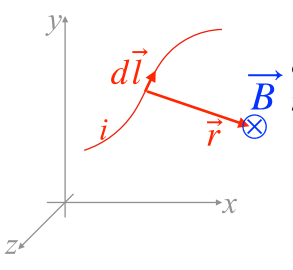
\includegraphics[scale=0.45]{img/Prima_legge_Laplace}
\par\end{center}

Dato che $i\text{d}\vec{l}=\vec{j}\text{d}\tau=nq\vec{v}_{d}\text{d}\tau=Nq\vec{v}_{d}$
allora possiamo riscrivere la formula precedente in relazione a $N$
cariche.

Dunque una singola carica in movimento genera un campo magnetico $\vec{B}$
che a distanza $r$ dalla carica stessa vale:

\[
\vec{B}=\frac{\mu_{0}}{4\pi}q\frac{\vec{v}_{d}\wedge\hat{r}}{r^{2}}=\frac{\mu_{0}}{4\pi}q\frac{\vec{v}_{d}\wedge\vec{r}}{r^{3}}
\]


\subsection*{Legge di Biot-Savart}

Il campo induzione magnetica generato da un filo rettilineo di lunghezza
indefinita, percorso da corrente $i$ è:

\[
\vec{B}=\frac{\mu_{0}i}{2\pi r}\hat{t}
\]

tangente alle circonferenze normali al filo.

\subsection*{Campi magnetici da cariche puntiformi in moto}

Consideriamo il campo elettrico generato da una singola carica $\vec{E}=\frac{q}{4\pi\varepsilon_{0}}\frac{\vec{r}}{r^{3}}\Rightarrow\frac{q\vec{r}}{r^{3}}=4\pi\varepsilon_{0}\vec{E}$.
Se andiamo a sostituire nella formula del campo magnetico generato
da una carica $\vec{B}=\frac{\mu_{0}}{4\pi}q\frac{\vec{v}\wedge\vec{r}}{r^{3}}$
ricaviamo:

\[
\vec{B}=\mu_{0}\varepsilon_{0}\vec{v}\wedge\vec{E}=\frac{1}{c^{2}}\vec{v}\wedge\vec{E}
\]

$c$ è la velocità della luce nel vuoto ed è legata alla costante
dielettrica e alla costante di permeabilità magnetica nel vuoto mediante
la formula $c=\frac{1}{\sqrt{\mu_{0}\varepsilon_{0}}}$.

\subsection*{Flusso del campo magnetico}

Per il teorema della divergenza, il flusso del campo magnetico attraverso
una qualsiasi \uline{superficie chiusa} sarà nullo: 
\[
\underset{S_{\text{chiusa}}}{\oiint}\vec{B}\cdot\hat{n}\text{d}S=0\qquad\underset{S_{\text{aperta}}}{\oiint}\vec{B}\cdot\hat{n}\text{d}S\in\mathbb{R}
\]


\subsection*{Circuitazione del campo magnetico}

La circuitazione lungo una linea chiusa e orientata $\Gamma$ che
concatena il filo:

\[
\underset{\Gamma}{\oint}\vec{B}\cdot\text{d}\vec{l}=\int_{0}^{2\pi}\frac{\mu_{0}i}{2\pi}\text{d}\phi=\pm\mu_{0}i
\]

La circuitazione lungo una linea chiusa e orientata $\Gamma$ che
non concatena il filo:

\[
\underset{\Gamma}{\oint}\vec{B}\cdot\text{d}\vec{l}=0
\]


\subsection*{Legge di Ampère}

La circuitazione del campo magnetico è proporzionale alla somma delle
correnti concatenate:

\[
\underset{\Gamma}{\oint}\vec{B}\cdot\text{d}\vec{l}=\mu_{0}\sum_{k}^{\text{conc.}}i_{k}
\]

\begin{center}
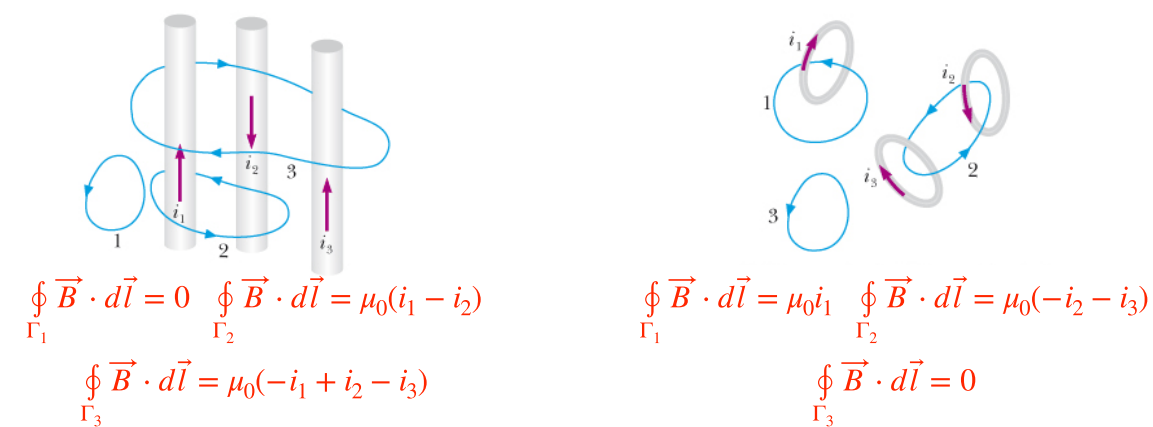
\includegraphics[scale=0.45]{img/Legge_di_Ampere}
\par\end{center}

\subsection*{Densità di corrente concatenata (Legge di Ampère in forma locale)}

Ciascuna corrente $i_{k}$ può essere scritta in funzione della densità
di corrente $i_{k}=\iint\vec{j}_{k}\cdot\hat{n}_{k}\text{d}S_{k}$
quindi:

\[
\underset{\Gamma}{\oint}\vec{B}\cdot\text{d}\vec{l}=\mu_{0}\iint_{S}\vec{j}_{\text{conc.}}\cdot\hat{n}\text{d}S\quad\equiv\quad\vec{\nabla}\wedge\vec{B}=\mu_{0}\vec{j}
\]

\pagebreak{}

\subsection*{Magnetismo della materia}

Se riempiamo la parte interna di un solenoide rettilineo ideale si
osserva una variazione del campo magneitico:
\begin{center}
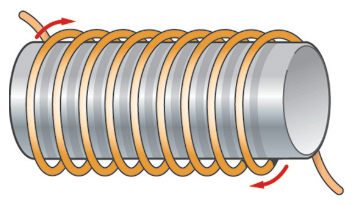
\includegraphics[scale=0.35]{img/Magnetismo_della_materia}
\par\end{center}
\begin{itemize}
\item materiali \textbf{diamagnetici} $\rightarrow$ leggera diminuzione
\item materiali \textbf{paramagnetici} $\rightarrow$ leggero aumento
\item materiali \textbf{ferromagnetici} $\rightarrow$considerevole aumento
\end{itemize}
Per spiegare il magnetismo nella materia occorre partire dalla struttura
microscopica semplificata (atomo idrogeno):
\begin{center}
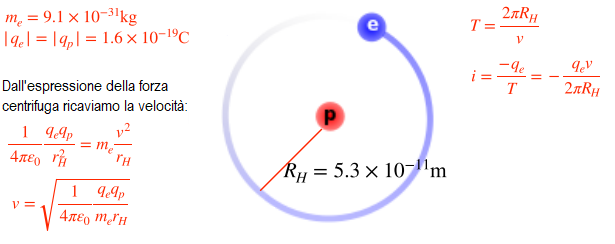
\includegraphics[scale=0.6]{img/Atomo_di_idrogeno}
\par\end{center}

\[
\text{Momento angolare orbitale }\vec{p}_{o}=\vec{R}_{H}\wedge m_{e}\vec{v}
\]

\[
\text{\textbf{Momento magnetico orbitale} }\vec{m}_{o}=iS=-\frac{q_{e}v}{2}R_{H}=-\frac{q_{e}}{2m_{e}}\vec{p}_{o}
\]

\[
\text{\textbf{Momento magnetico di spin} }\vec{m}_{s}=-\frac{q_{e}}{m_{e}}\vec{p}_{s}
\]

Il \textbf{momento magnetico totale} o instrinseco ($\vec{m}$) dato
dall'accoppiamento tra momento magnetico orbitale e di spin, in un
generico atomo, dipende dagli elettroni più esterni e in assenza di
campi magnetici esterni esso \uline{è macroscopicamente nullo}
perchè i momenti magnetici degli atomi sono orientati casualmente
e la loro somma vettoriale è nulla.

\subsection*{Materiali diamagnetici}

In questi materiali, l’effetto di un campo esterno è quello di deviare
la traiettoria degli elettroni in moto, inducendo una variazione di
velocità (l’elettrone si allontana dal nucleo) e quindi una diminuzione
della frequenza di rotazione (precessione di Larmor).

L’effetto complessivo è una diminuzione del momento magnetico, che
va ad opporsi leggermente al campo magnetico esterno.

$\,$

I materiali diamagnetici in genere hanno un numero pari di elettroni
e struttura simmetrica.

\subsection*{Materiali paramagnetici}

I materiali paramagnetici hanno atomi con momento angolare totale
diverso da zero.

Gli atomi si comportano come dipoli magnetici che per effetto di un
campo magnetico esterno tendono ad allinearsi con il campo magnetico
esterno, contribuendo ad aumentarne leggermente il valore.

$\,$

I materiali paramagnetici sono caratterizzati da un numero dispari
di elettroni o da strutture atomiche asimmetriche.

\subsection*{Materiali ferromagnetici}

I materiali ferromagnetici microscopicamente hanno una configurazione
elettronica per cui si creano forti interazioni tra momenti orbitali
e momenti di spin. Tali interazioni comportano che momenti magnetici
di atomi adiacenti si “accoppiano”, aumentando considerevolmente il
loro effetto magnetico rispetto al singolo atomo All’interno del materiale
si creano regioni formate da numerosi dipoli allineati (domini di
Weiss).
\begin{center}
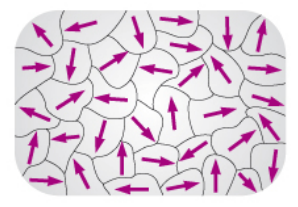
\includegraphics[scale=0.4]{img/Materiali_ferromagnetici}
\par\end{center}

Quando un materiale ferromagnetico viene posto in un campo magnetico
esterno i momenti si allineano con il campo magnetico, generando una
fusione dei domini di Weiss
\begin{center}
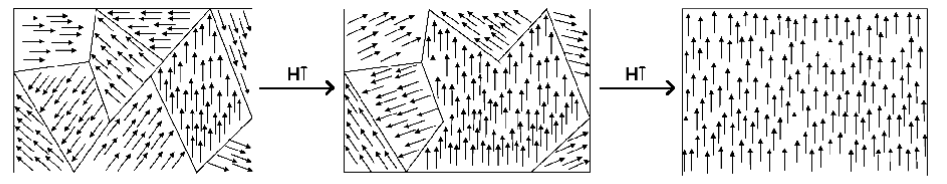
\includegraphics[scale=0.4]{img/Materiali_ferromagnetici2}
\par\end{center}

I domini di Weiss vengono distrutti se il materiale viene riscaldato
fino ad una temperatura critica (di Curie), per cui l'interazione
tra gli atomi è maggiore dei momenti magnetici e dunque il materiale
non risultà più magnetizzato ma si comporta come un materiale paramagnetico.

$\,$

Ponendo campi magnetici sempre più intensi, si arriva ad una condizione
di saturazione cioè il materiale mantiene una magnetizzazione residua
anche fuori dal campo magnetico. 
\begin{center}
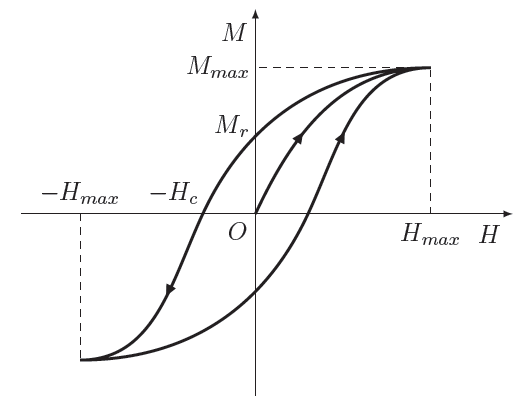
\includegraphics[scale=0.35]{img/Isteresi_campo_magnetico}
\par\end{center}

Come si può osservare dall'immagine (ciclo di isteresi per un campo
magnetico) in primo momento in cui si ha campo magnetico e magnetizzazione
del materiale nulla, se si aumenta il campo magnetico, il materiale
si magnetizza aumentando proporzionalmente con il campo e raggiunge
il suo massimo valore detto \textbf{valore di saturazione}\@. Diminuendo
il campo magnetico fino ad azzerarlo, il materiale mantiene una magnetizzazione
residua.

\subsection*{Vettore magnetizzazione}

Definiamo il vettore magnetizzazione come il prodotto del momento
angolare intrinseco medio del materiale per il numero di atomi per
unità di volume:

\[
\vec{M}=n\left\langle \vec{m}\right\rangle =\frac{N}{\text{d}\tau}\left\langle \vec{m}\right\rangle 
\]


\subsection*{Vettore H}

Definiamo il vettore $H$ che descrive il campo magnetico nella materia,
in funzione solo delle correnti di conduzione

\[
\vec{H}=\frac{\vec{B}}{\mu_{0}}-\vec{M}
\]

Proprietà:

\[
\vec{\nabla}\wedge\vec{H}=\vec{j}\qquad\qquad\vec{B}=\mu_{0}\vec{H}+\mu_{0}\vec{M}
\]

\pagebreak{}

\section{Campi elettrici e magnetici variabili nel tempo}

\subsection*{Equazioni di Maxwell (forma integrale)}
\begin{center}
\begin{tabular}{cc}
\hline 
\multicolumn{1}{|c|}{\textbf{Campo elettrico}} & \multicolumn{1}{c|}{\textbf{Campo magnetico}}\tabularnewline
\hline 
\uline{Legge di Gauss} & \uline{Legge di Gauss}\tabularnewline
$\Phi_{S}\left(\vec{E}\right)=\underset{S}{\oiint}\vec{E}\cdot\hat{n}\text{d}S=\frac{Q_{S}}{\varepsilon_{0}}$ & $\underset{S}{\oiint}\vec{B}\cdot\hat{n}\text{d}S=0$\tabularnewline
Conservatività & \uline{Legge di Ampère}\tabularnewline
$\underset{\Gamma}{\oint}\vec{E}\cdot\text{d}\vec{l}=0$ & $\underset{\Gamma}{\oint}\vec{B}\cdot\text{d}\vec{l}=\mu_{0}{\displaystyle \sum_{k}^{\text{conc.}}i_{k}}$\tabularnewline
\end{tabular}
\par\end{center}

\subsection*{Equazioni di Maxwell (forma differenziale)}
\begin{center}
\begin{tabular}{cc}
\hline 
\multicolumn{1}{|c|}{\textbf{Campo elettrico}} & \multicolumn{1}{c|}{\textbf{Campo magnetico}}\tabularnewline
\hline 
\uline{Legge di Gauss} & \uline{Legge di Gauss}\tabularnewline
$\vec{\nabla}\cdot\vec{E}=\frac{\rho}{\varepsilon_{0}}$ & $\vec{\nabla}\cdot\vec{B}=0$\tabularnewline
Conservatività & \uline{Legge di Ampère}\tabularnewline
$\vec{\nabla}\wedge\vec{E}=0$ & $\vec{\nabla}\wedge\vec{B}=\mu_{0}\vec{j}$\tabularnewline
\end{tabular}
\par\end{center}

\subsection*{Legge di Ampère-Maxwell}

Il campo magnetico può essere generato da cariche in moto e da campi
elettrici variabili nel tempo.

La legge di Ampère-Maxwell è valida sempre, sia in regime stazionario
che non stazionario. Infatti la divergenza della somma dei termini
di densità di corrente di spostamento e conduzione è sempre nulla.

\[
\vec{\nabla}\wedge\vec{B}=\mu_{0}\vec{j}+\mu_{0}\varepsilon_{0}\frac{\partial\vec{E}}{\partial t}
\]

\[
\underset{\Gamma}{\oint}\vec{B}\cdot\text{d}\vec{l}=\mu_{0}\sum_{k}^{\text{conc.}}\left(i_{c}+i_{s}\right)
\]


\subsection*{Legge di Faraday-Neumann-Lenz}

La variazione temporale del flusso di un campo magnetico “induce”
una forza elettromotrice, la quale è opposta alla variazione del flusso
che l’ha generata

\[
\mathscr{E}_{\text{ind.}}=-\frac{\text{d}}{\text{d}t}\iint_{S}\vec{B}\cdot\hat{n}\text{d}S=-\frac{\text{d}\Phi_{S}\left(\vec{B}\right)}{\text{d}t}
\]

Osservazione: La superficie deve essere aperta altrimenti per il teorema
di Gauss del campo magnetico il flusso è nullo.

\[
\vec{\nabla}\wedge\vec{E}=-\frac{\partial\vec{B}}{\partial t}
\]


\subsection*{Induzione}

Poichè per la prima legge di Laplace il campo magnetico dipende linearmente
dalla corrente allora anche il flusso del campo magnetico sarà proporzionale
alla corrente:

\[
\Phi\left(\vec{B}\right)=Mi
\]

Dove $M$ è detto \textbf{coefficiente di mutua induzione} e dipende
solamente dalla forma del circuito percorso da corrente. Nel S.I si
misura in Henry.

Per la legge di Faraday-Neumann-Lenz:

\[
\mathscr{E}_{\text{ind.}}=-\frac{\text{d}\Phi_{S}\left(\vec{B}\right)}{\text{d}t}=-M\frac{\text{d}i}{\text{d}t}
\]


\subsection*{Autoinduzione}

Un circuito percorso da corrente variabile nel tempo genera un campo
magnetico variabile nel tempo che comporta un flusso variabile nel
tempo

\[
\Phi\left(\vec{B}\right)=Li
\]

Dove $L$ è detto \textbf{coefficiente di autoinduzione} (o \textbf{induttanza})
e dipende solamente dalla forma del circuito percorso da corrente.
Nel S.I. di misura in Henry.

Per la legge di Faraday-Neumann-Lenz:

\[
\mathscr{E}_{\text{ind.}}=-\frac{\text{d}\Phi_{S}\left(\vec{B}\right)}{\text{d}t}=-L\frac{\text{d}i}{\text{d}t}
\]


\subsection*{Induttanza}

\subsubsection*{Esempio induttanza di un solenoide cilindrico ideale}

L'induttanza di un solenoide cilindrico ideale di lunghezza $l$ formato
da $N$ spire di raggio $r$ vale:

\[
L=\frac{\Phi_{\text{solenoide}}\left(\vec{B}\right)}{i\left(t\right)}=\frac{N\Phi_{\text{spira}}\left(\vec{B}\right)}{i\left(t\right)}=\frac{N\mu_{0}\frac{N}{l}i\left(t\right)\pi r^{2}}{i\left(t\right)}=\mu_{0}\frac{N^{2}}{l}S\qquad S=\pi r^{2}
\]

\begin{center}
\textbf{Induttanze in serie}
\par\end{center}

\begin{center}
Nella connessione in serie gli elementi circuitati sono attraversati
dalla \uline{stessa corrente}.
\par\end{center}

\[
L_{\text{TOT}}=\Sigma L_{i}
\]

\begin{center}
\textbf{Induttanze in parallelo}
\par\end{center}

\begin{center}
Nella connessione in parallelo gli elementi circuitati sono alla \uline{stessa
differenza di potenziale}.
\par\end{center}

\[
\frac{1}{L_{\text{TOT}}}=\Sigma\frac{1}{L_{i}}
\]


\subsubsection*{Energia magnetica}

Per spostare la carica all'interno dell'induttanza occorre contrastare
la fem autoindotta, cioè occorre fare un lavoro contro la fem autoindotta.

Il lavoro per aumentare la corrente di un valore $\text{d}i$ è:

\[
\delta\mathscr{L}=-\mathscr{E}_{\text{autoindotta}}\text{d}q=-\left(-L\frac{\text{d}i}{\text{d}t}\right)i\text{d}t
\]

Se iniziamente nell'induttanza non circola corrente $i\left(0\right)=0$,
per portare il circuito a corrente $i$ occorre compiere un lavoro:

\[
\mathscr{L}=\int_{0}^{i}Li\text{d}i=\frac{1}{2}Li^{2}
\]

Il lavoro accumula energia nell'induttanza. Essendo $L=\mu_{0}\frac{N^{2}}{l}S$
e $B=\mu_{0}\frac{N}{l}i\Rightarrow i=\frac{Bl}{\mu_{0}N}$

\[
U_{B}=\frac{1}{2}Li^{2}=\frac{B^{2}}{2\mu_{0}}\left(lS\right)=\frac{B^{2}}{2\mu_{0}}\text{V}_{\text{solenoide}}=\underset{\text{spazio}}{\iiint}u_{B}\text{d}\tau
\]


\subsubsection*{Densità di energia magnetica}

\[
u_{B}=\frac{B^{2}}{2\mu_{0}}
\]


\subsection*{Circuiti RL in regime transitorio}

\subsubsection*{Carica di un induttore}
\begin{center}
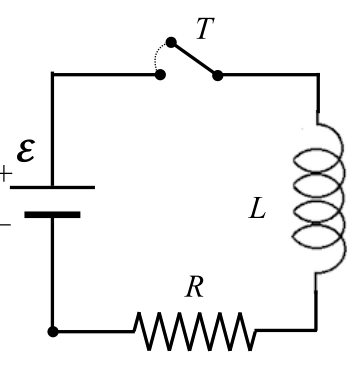
\includegraphics[scale=0.35]{img/Circuito_RL}
\par\end{center}

Nel momento in cui si va a chiudere l'interruttore l'equazione alla
maglia diventa: 

\[
\mathscr{E}+\mathscr{E}_{\text{ind.}}=\mathscr{E}-L\frac{\text{d}i}{\text{d}t}=Ri\Rightarrow\frac{\text{d}i}{\text{d}t}=-\frac{R}{L}\left(i-\frac{\mathscr{E}}{R}\right)\Rightarrow\frac{\text{d}i}{\left(i-\frac{\mathscr{E}}{R}\right)}=-\frac{R}{L}\text{d}t
\]

\[
\int_{i\left(0\right)}^{i\left(t\right)}\frac{\text{d}i}{\left(i-\frac{\mathscr{E}}{R}\right)}=\int_{0}^{t}-\frac{R}{L}\text{d}t\Rightarrow\left[\ln\left(i-\frac{\mathscr{E}}{R}\right)\right]_{i\left(0\right)}^{i\left(t\right)}=-\frac{R}{L}t\Rightarrow\ln\left(\frac{i-\frac{\mathscr{E}}{R}}{-\frac{\mathscr{E}}{R}}\right)=-\frac{R}{L}t\Rightarrow i-\frac{\mathscr{E}}{R}=-\frac{\mathscr{E}}{R}e^{-\frac{R}{L}t}
\]

\[
i\left(t\right)=\frac{\mathscr{E}}{R}\left(1-e^{-\frac{R}{L}t}\right)
\]

In regime stazionario $\left(t\rightarrow\infty\right)$:
\begin{itemize}
\item $\mathscr{E}_{\text{ind.}}=-L\frac{\text{d}i}{\text{d}t}=-\mathscr{E}e^{-\frac{R}{L}t}\underset{t\rightarrow\infty}{\longrightarrow}0$
\item L'induttanza si comporta come un filo a resistenza nulla
\item Nell'induttanza vi è immagazzinata un'energia magnetica $U_{B}=\frac{1}{2}Li^{2}$
\end{itemize}

\subsubsection*{Scarica di un induttore}
\begin{center}
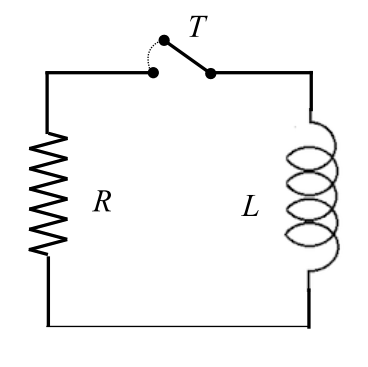
\includegraphics[scale=0.35]{img/Scarica_induttore}
\par\end{center}

\[
\mathscr{E}_{\text{ind.}}=-L\frac{\text{d}i}{\text{d}t}=Ri\Rightarrow\frac{\text{d}i}{\text{d}t}=-\frac{R}{L}i\Rightarrow\frac{\text{d}i}{i}=-\frac{R}{L}\text{d}t
\]

\[
\int_{i\left(0\right)}^{i\left(t\right)}\frac{\text{d}i}{i}=\int_{0}^{t}-\frac{R}{L}\text{d}t\Rightarrow\left[\ln\left(i\right)\right]_{i\left(0\right)}^{i\left(t\right)}=-\frac{R}{L}t\Rightarrow\frac{i\left(t\right)}{i\left(0\right)}=e^{-\frac{R}{L}t}
\]

\[
i\left(t\right)=i\left(0\right)e^{-\frac{R}{L}t}
\]

\begin{itemize}
\item La corrente iniziale si ricava dalla condizione iniziale di energia
immagazzinata nell'induttanza:
\end{itemize}
\[
U_{B}=\frac{1}{2}Li\left(0\right)^{2}\Rightarrow i\left(0\right)=\sqrt{\frac{2U_{B}}{L}}
\]

\begin{itemize}
\item Tutta l'energia accumulata nell'induttanza viene dissipata per effetto
Joule sulla resistenza
\end{itemize}

\end{document}
